\documentclass[12pt,a4paper,oneside,openany]{article}

\usepackage{textcase}
\usepackage{indentfirst}
\usepackage[]{graphicx}
\usepackage{subcaption}
\usepackage{booktabs}
\usepackage{setspace}\onehalfspacing\frenchspacing

%\linespread{1.3}

%Russian-specific packages
\usepackage[T2A]{fontenc}
\usepackage[utf8]{inputenc}
\usepackage[russian]{babel}

\usepackage{hyperref}
\usepackage{xcolor}

\newcommand{\FIXME}[1]{ % описание
	\colorbox{yellow}{FIXME:} #1
}

%algorithms
\usepackage{float}
\usepackage[boxed,vlined,ruled]{algorithm2e}
\renewcommand{\algorithmcfname}{Алгоритм}

%code
\usepackage{listings}

% sections
\usepackage{tocloft}
\renewcommand{\cftdot}{}
%\renewcommand{\cftsecleader}{\cftdotfill{\cftdotsep}}
\renewcommand{\thesection}{\arabic{section}}

\usepackage{lipsum}
\usepackage[margin=2cm,left=3cm,right=15mm,includefoot]{geometry}

% theorems
\usepackage{amsthm}
\newtheorem{theorem}{Теорема}

\theoremstyle{definition}
\newtheorem{definition}{Определение}[]

\theoremstyle{lemma}
\newtheorem{lemma}{Утверждение}[]

\theoremstyle{remark}
\newtheorem{remark}{Замечание}[]

\begin{document}
\begin{titlepage}
        \begin{center}

        \bigskip

        \MakeTextUppercase{Московский государственный университет им. М.В. Ломоносова} \\

        \MakeTextUppercase{Факультет вычислительной математики и кибернетики} \\
        \MakeTextUppercase{Кафедра суперкомпьютеров и квантовой информатики} \\
        \bigskip

        
\includegraphics[width=50mm]{msu.eps}

        \bigskip
        \bigskip
        \MakeTextUppercase{\textbf{\Huge Магистерская диссертация}} \\
        \bigskip
        {\large на тему:} \\
        \bigskip
        \MakeTextUppercase{\textbf{\large Алгоритмы поиска подграфов типа <<черная дыра>> в ориентированном графе}}

        \bigskip
        Шифр и наименование специальности

    \end{center}

    \bigskip
    \bigskip
    \bigskip
    \begin{flushright}
        \begin{minipage}{7cm}
            \textbf{Выполнил:} \\
            студент гр. М-218 \\
            Иванов Денис Евгеньевич \\

            \textbf{Научный руководитель:} \\
            к.т.н. Семенов Александр Сергеевич \\

            \textbf{Рецензент:} \\
            ??????? ??????? ???????
        \end{minipage}
    \end{flushright}

    \vfill

    \begin{center}
    {\large Москва, 2020}
    \end{center}

\end{titlepage}

\setcounter{page}{2}

\setcounter{tocdepth}{2}
\tableofcontents
\addcontentsline{toc}{section}{Содержание}

\cleardoublepage
\section{Введение}\label{sec:otherintro}

Одним из важных свойств графов, которые описывают объекты реального мира,
является присутствие в них кластеров или сообществ.

Задача поиска этих сообществ имеет важное значение в социологии, биологии и компьютерных науках,
поскольку объекты, изучаемые в данных прикладных областях, часто естественно моделируются при
помощи графов \cite{fortunato2010community}.

В работе \cite{li2010detecting} впервые сформулирована задача поиска подграфов (паттернов) типа <<черная дыра>> и <<вулкан>> ориентированных графах. В соответствии с этой работой, черная дыра -- множество вершин графа, в которого отсутствуют исходящие ребра. Вулкан -- это, наоборот, множество вершин графа, у которого имеются только исходящие ребра.

Паттерны черная дыра и вулкан встречаются в прикладных задачах. Например, в торговой сети, паттерн черная дыра может представлоять собой группу торговцев, которые манипулируют рынком. Также черная дыра и вулкан могут описывать собой схемы отмывания денег \cite{semenov2017survey}. Поиск черных дыр и вулканов в реальном времени может  своевременно обнаружить пагубные явления, такие как природные катаклизмы, катастрофы, происшествия. Разработка алгоритмов поиска таких паттернов позволяет сохранять общественную безопасность \cite{hong2015detecting}.

Основной вклад в исследование задачи поиска паттерна черная дыра внесла группа авторов из университета Нью-Джерси. Они сформулировали задачу и предложили алгоритм поиска черных дыр в случае невзвешенного ориентированного графа \cite{li2010detecting}. Два  года спустя эти же авторы опубликовали алгоритм для приближенного поиска черных дыр в случае взвешенного графа \cite{li2012mining,li2014mining}. Hong \cite{hong2015detecting} рассматривает задачу поиска черных дыр в реальном времени для  нужд современного города. В этой работе предлагается оригинальный алгоритм, приближенно решающий задачу для динамических графов. Другие работы, посвященные поиску паттерна <<черная дыра>> в графе, автору данной работы неизвестны. 

\FIXME{Необходимо автоматически проверить текст на грамотность}

В данной работе рассматриваеся упрощенная постановка задачи поиска черных дыр для случая ориентированного графа без весов.

\cleardoublepage
\section{Постановка задачи}\label{sec:taskstatement}

\FIXME{Здесь и далее вместо дефиса (одна черточка -) нужно тире (две черточки --)}

Рассмотрим граф $G = G(V,E)$, где $V$ - множество вершин, а $E$ - множество ребер.

\begin{definition}\label{def:blackhole}
Подмножество вершин $B \subseteq V$ называется черной дырой, если одновременно выполняются следующие условия: 1) подграф $G'(B,E')$ слабо связан и 2) нет такой пары вершин $(u,v)$ что $u \in B,\ v \in V\setminus{B};\ (u,v) \in E$.
\end{definition}

Задача состоит в том, чтобы в ориентированном графе без весова найти как можно больше черных дыр (или рассмотреть максимальное количество кандидатов) за ограниченное время.

\FIXME{Здесь необходимо сформулировать задачи исследования, примерно как в презентации.}

\cleardoublepage

\section{Существующие алгоритмы решения задачи поиска черных дыр в графе}\label{sec:prevsolutions}

\subsection{Определения}\label{sec:definitions}

Введем несколько дополнительных определений.

\begin{definition}\label{def:orpath}
	Пусть дан ориентированный граф $G(V,E)$. Последовательность $v_0v_1v_2...v_k$, состоящая из вершин $v_i \in V,\ 0 \leq i \leq k$ образует ориентированный путь из $v_0$ в $v_k$, если существуют ребра $(v_{i-1}, v_i) \in E,\ 1 \leq i \leq k$ и $v_i \neq v_j$ для всех $0 \leq i,\ j \leq k,\ i \neq j$. Длина такого ориентированного пути равна $k$.
\end{definition}

\begin{definition}\label{def:reachablevertex}
	Пусть дан ориентированный граф $G(V,E)$. Вершина $v \in V$ достижима из $u \in V$, если существует ориентированный путь, который начинается в $u$ и заканчивается в $v$.
\end{definition}

\begin{definition}\label{def:successor}
	Пусть дан ориентированный граф $G(V,E)$. Если вершина $v \in V$ достижима из $u \in V$ тогда $u$ является ориентированным предком $v$, а $v$ является ориентированным потомком $u$. Если существует ребро из $u$ в $v$, то $u$ является непосредственным предком $v$ , а $v$ является непосредственным потомком $u$.
\end{definition}

\begin{definition}\label{def:scc}
	Подмножество вершин $B \subseteq G$ называется компонентой сильной связности (КСС), если все вершины $B$ попарно взаимно достижимы.
\end{definition}

\begin{definition}\label{def:closure}
	Пусть дан ориентированный граф $G(V,E)$. Рассмотрим вершину $v \in V$. Замыкание вершины $Closure(v)\ =\ \{u\ |\ u$ достижима из $v\} \cup {v}$.
	Другими словами, замыкание вершины $v$ --- это множество всех вершин, достижимых из $v$, включая ее саму.
\end{definition}

Следующие утверждения были ранее доказаны в статье \cite{li2010detecting}.

\begin{lemma}
	Если вершина $v \in B$, причем $B \subseteq V$ --- черная дыра, то все потомки $v$ лежат в $B$.
\end{lemma}

\begin{lemma}
	Если вершина $v \in B$, причем $B \subseteq V$ --- черная дыра, то замыкание $v$ полностью содержится в $B$.
\end{lemma}

\begin{lemma}\label{lemma:closurebh}
	Замыкание любой вершины образует черную дыру.
\end{lemma}


\subsection{Алгоритм BruteForce}\label{subsec:bruteforce}

\linespread{1.0}
\begin{figure}[H]
	\begin{center}
		\begin{algorithm}[H]
			\SetAlgoLined
			\SetKwInOut{Input}{Input}
			\SetKwInOut{Output}{Output}
			\Input{$G(v, E)$ -- ориентированный граф, $V$ -- множество вершин, $E$ -- множество ребер, \\
                   $n$ -- максимальное число вершин, которое может содержать черная дыра}
			\Output{$Blackholes$ -- множество всех черных дыр графа размером от 1 до n}

                        $Blackholes = \emptyset, C_0 = \emptyset$ \\
                        \For{$i = 1\ to\ n$} {
                            \ForEach{$B \in V(i)$} {
                                \If{$G(B)$ -- слабо связан} {
                                    \If{$d_{out}(B) == 0$} {
                                        $Blackholes = Blackholes \cup B$
                                    }
                                }
                            }
                        }
                        \Return $Blackholes$
			\label{alg:bruteforce}
			\caption{BruteForce}
		\end{algorithm}
	\end{center}
\end{figure}
\linespread{1.5}

\FIXME{Английские названия алгоритмов не принято ставить в кавычки}

\FIXME{Все кавычки "" в тексте лучше заменить на елочки <<>>}

Наиболее простым способом решения задачи является алгоритм \ref{alg:bruteforce} BruteForce.
Он заключается в последовательном переборе наборов вершин размером от 1 до N.
Каждый набор проверяется на соответствию определению черной дыры (см. Опред. \ref{def:blackhole}).
Проверяется наличие свойства слабой связности, а затем и наличие исходящих ребер.
Такой подход никак не учитывает особенности внутреннего устройства черных дыр при переборе и поэтому рассматривает большое количество избыточных вариантов.
В частности, необходимости рассматривать наборы, которые заведомо имеют исходящие ребра, можно избежать, что будет продемонстрировано позже.

\subsection{Алгоритм iBlackhole}\label{subsec:iblackhole}

В 2010 году в статье \cite{li2010detecting} был предложен алгоритм iBlackhole.

\linespread{1.0}
\begin{figure}[H]
	\begin{center}
		\begin{algorithm}[H]
			\SetAlgoLined
			\SetKwInOut{Input}{Input}
			\SetKwInOut{Output}{Output}
			\Input{$G(v, E)$ -- ориентированный граф, $V$ -- множество вершин, $E$ -- множество ребер, \\
                   $n$ -- максимальное число вершин, которое может содержать черная дыра}
			\Output{$Blackholes$ -- множество всех черных дыр графа размером от 1 до n}

                        $Blackholes = \emptyset, C_0 = \emptyset$ \\
                        \For{$i = 1\ to\ n$} {
                            $P_i = \{v | d_{out}(v) < i\}$
                            \tcp*[f]{$d_{out}(v)$ количество исходящих из $v$ ребер} \\
                            \ForEach{$v \in P_i$} {
                                \If{$v \notin C_{i-1}$} {
                                    \If{как минимум один из непосредственных потомков $v$ не принадлежит $P_i$} {
                                        удалить $v$ из $P_i$\\
                                        удалить вcех предков $v$ из $P_i$ \\
                                    }
                                }
                            }
                            $C_i = P_i$  \tcp*[f]{$C_i$ -- список кандидатов} \\
                            \ForEach{$v \in C_i$} {
                                \If{$|Closure(v)| == i$} {
                                    $Blackholes = Blackholes \cup Closure(v)$
                                }
                                \If{$|Closure(v)| >= i$} {
                                    удалить $v$ из $С_i$\\
                                    удалить вcех предков $v$ из $С_i$ \\
                                }
                            }
                            \tcc{Применить алгоритм полного перебора к $F_i(i)$ -- множеству всех подмножеств $F_i$, содержащих $i$ вершин}
                            \ForEach{$B \in F_i(i)$} {
                                \If{$G(B)$ -- слабо связан} {
                                    \If{$d_{out}(B) == 0$} {
                                        $Blackholes = Blackholes \cup B$ \\
                                    }
                                }
                            }
                        }
                        \Return $Blackholes$
			\label{alg:iblackhole}
			\caption{iBlackhole}
		\end{algorithm}
	\end{center}
\end{figure}
\linespread{1.5}

\FIXME{Слово "заточен" неформально}
 
Алгоритм \ref{alg:iblackhole} заточен для поиска черных дыр заданного размера, но также позволяет найти в графе черные дыры всех размеров.
Идея авторов из университета Нью-Джерси состоит в том, чтобы на каждой итераиции исключать из рассмотрения вершины, которые заведомо не могут
образовывать черные дыры заданного размера, тем самым сокращая перебор.
К вершинам, которые прошли фильтр на данной итерации, применяется алгоритм BruteForce, описанный выше.
Итерации алгоритма идут по возрастанию размера черных дыр. Это позволяет постепенно наращивать размер множества кандидатов.

\linespread{1.0}
\begin{figure}[H]
	\begin{center}
		\begin{algorithm}[H]
			\SetAlgoLined
			\SetKwInOut{Input}{Input}
			\SetKwInOut{Output}{Output}
			\Input{$G(v, E)$ -- ориентированный граф, $V$ -- множество вершин, $E$ -- множество ребер, \\
                   $n$ -- максимальное число вершин, которое может содержать черная дыра}
			\Output{$Blackholes$ -- множество всех черных дыр графа размером от 1 до n}

                        $Blackholes = \emptyset, C_0 = \emptyset$ \\
                        \For{$i = 1\ to\ n$} {
                            $P_i = \{v | d_{out}(v) < i\}$ \\
                            убрать лишние вершины из $P_i$ и сформировать список кандидатов $C_i$ \\
                            убрать лишние вершины из $C_i$ и сформировать список кандидатов $F_i$ \\
                            \ForEach{$WCC \in G(F_i)$} {
                                \tcc{Применить алгоритм полного перебора к $WCC_i(i)$ -- множеству всех подмножеств $WCC_i$, содержащих $i$ вершин}
                                \ForEach{$B \in WCC_i(i)$} {
                                    \If{$G(B)$ -- слабо связан} {
                                        \If{$d_{out}(B) == 0$} {
                                            $Blackholes = Blackholes \cup B$
                                        }
                                    }
                                }
                            }
                        }
                        \Return $Blackholes$
			\label{alg:iblackholedc}
			\caption{iBlackholeDC}
		\end{algorithm}
	\end{center}
\end{figure}
\linespread{1.5}

В той же работе авторы предлагают модификацию алгоритма: iBlackholeDC. DC здесь означает <<Divide and Conquer>>, т.е. <<Разделяй и Властвуй>>.
На стадии полного перебора авторы предлагают рассматривать только наборы вершин полностью содержащиеся внутри компонент слабой связности
графа, индуцированного множеством кандидатов.
Это, само по себе, не гарантирует, что такой набор будет удовлетворять требованию слабой связности, но избавляет от необходимости
рассматривать заведомо несвязные наборы. Например, если рассмотрeть две вершины, находящиеся в разных компонентах слабой связности,
то между ними не найдется направленного пути.

Алгоритм iBlackholeDC хорошо работает для поиска небольших черных дыр в любых графах.
Если же граф не содержит черных дыр малого размера, или он содержит крупные компоненты сильной связности,
то алгоритм iBlackholeDC долгое время будет безрезультатно перебирать наборы вершин меньшего размера.
Так как алгоритм BruteForce используется как составная часть, то можно говорить о наследовании проблем
алгоритма BruteForce алгоритмом iBlackholeDC.

\subsection{Известные проблемы}\label{subsec:knownissues}

\FIXME{применимость к чему?}
В данном разделе рассматривается применимость алгоритма iBlackholeDC \cite{li2010detecting}.

Введем дополнительное утверждение, чтобы описать проблемы существующего подхода.

\begin{lemma}{}
Все вершины КСС принадлежат одной черной дыре.
\end{lemma}
\begin{proof}
В КСС все вершины попарно взаимно достижимы по определению.
Это значит, что замыкание произвольной вершины КСС содержит всю КСС как подмножество.
Опираясь на Лемму \ref{lemma:closurebh}, получаем, что КСС принадлежит той же черной дыре, что и вершина $v$.
\end{proof}

Рассмотрим следующий пример.
Граф состоит из $10^6$ вершин, которые образуют единую КСС.
Это значит, что в данном графе существует только одна черная дыра - это весь граф.
Если о структуре графа ничего не известно, а также нет достаточно больших вычислительных ресурсов,
возникает необходимость перебирать слишком большое число размеров черных дыр.
В худшем случае нам придется перебрать все возможные размеры множеств кандидатов.
В реальности, при использовании iBlackholeDC привется ждать слишком долго, чтобы в итоге получить тривиальный ответ.

Другой пример - это графы малого мира (SmallWorld) \cite{watts1999networks}.
Большая часть вершин такого графа содержится в единственной большой КСС.
Также имеется несколько вершин и корней.
Нетрудно проверить, что при просмотре от меньших размеров черной дыры к большим,
алгоритм iBlackhole быстро обнаружит все небольшие черные дыры.
Далее он будет очень долго пытаться найти черные дыры внутри КСС,
где их попросту нет, пока не доберется до размеров больше размера КСС.

Алгоритм iBlackholeDC:
    \begin{itemize}
        \item Неэффективно работает со SmallWorld графами;
        \item Каждую итерацию завершает перебором, часто просматривая заведомо неверные варианты;
        \item Не был испытан авторами на графах размером более 1500 вершин.
    \end{itemize}

\cleardoublepage
\section{Разработка алгоритмов поиска черных дыр в графе}\label{sec:topalgodesign}

\FIXME{Нужно переделать название этого раздела так, чтобы он описывал все, что сделано в этом разделе. Здесь не только топологический алгоритм. Предложил свой вариант (было -- Разработка топологического алгоритма)}

В данной работе предлагается предлагается рассмотреть решение задачи поиска черных дыр при помощи комбинации двух этапов.
Первый этап состоит в предобработке графа, задача которой упростить структуру графа.
Уменьшение размера графа значительно сокращает размер задачи. Это важно в силу комбинаторной природы задачи.
Второй этап - это непосредственно поиск черных дыр. Здесь не получится избежать перебора в том или ином виде,
однако этот перебор можно построить по-разному.
Целью данного этапа является обнаружение как можно большего числа черных дыр при заданном ограничении по времени.

\subsection{Предобработка графа}\label{subsec:graphpreprocessing}

Как было сказано выше, большие КСС требуют значительных вычислительных ресурсов для обработки и при этом не образуют дополнительных черных дыр.
Это может быть критично при обработке графов малого мира, потому что одна КСС может включать до 100\% вершин такого графа.
При работе с подобными графами будет удобно рассмотреть КСС как единую вершину,
которая объединяет в себе все входящие и исходящие связи периферических вершин КСС.
Процесс сжатия каждой КСС до единственной вершины известен под названием конденсация графа.

\begin{definition}\label{def:condensation}
Если каждую компоненту сильной связности заменить единственной вершиной, то получится ориентированный ациклический граф, который называется конденсацией исходного графа.
\end{definition}

В данной работе для поиска компонент сильной связности используется алгоритм Шарира \cite{sharir1981strong}.

Конденсированный граф имеет следующие свойства:
    \begin{itemize}
        \item Ориентированный;
        \item Без циклов;
        \item Размер меньше, чем исходный граф.
    \end{itemize}

\begin{figure}[H]
    \begin{subfigure}{.5\textwidth}
      \centering
      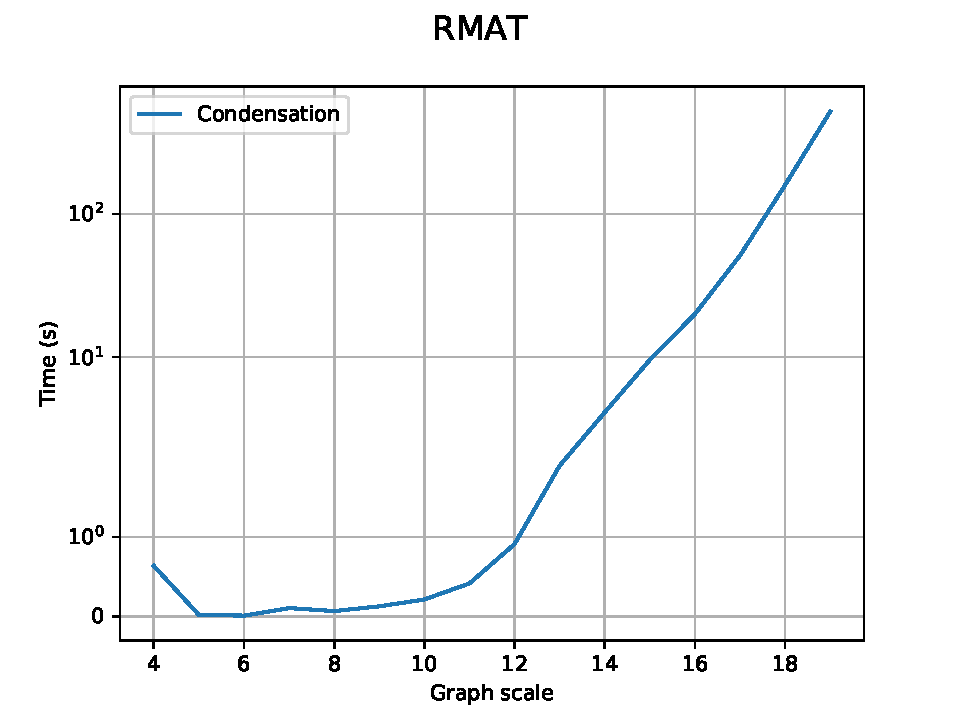
\includegraphics[width=8cm]{images/condensation_RMAT.pdf}
      \caption{RMAT}
      \label{fig:condensation:rmat}
    \end{subfigure}
    \begin{subfigure}{.5\textwidth}
      \centering
      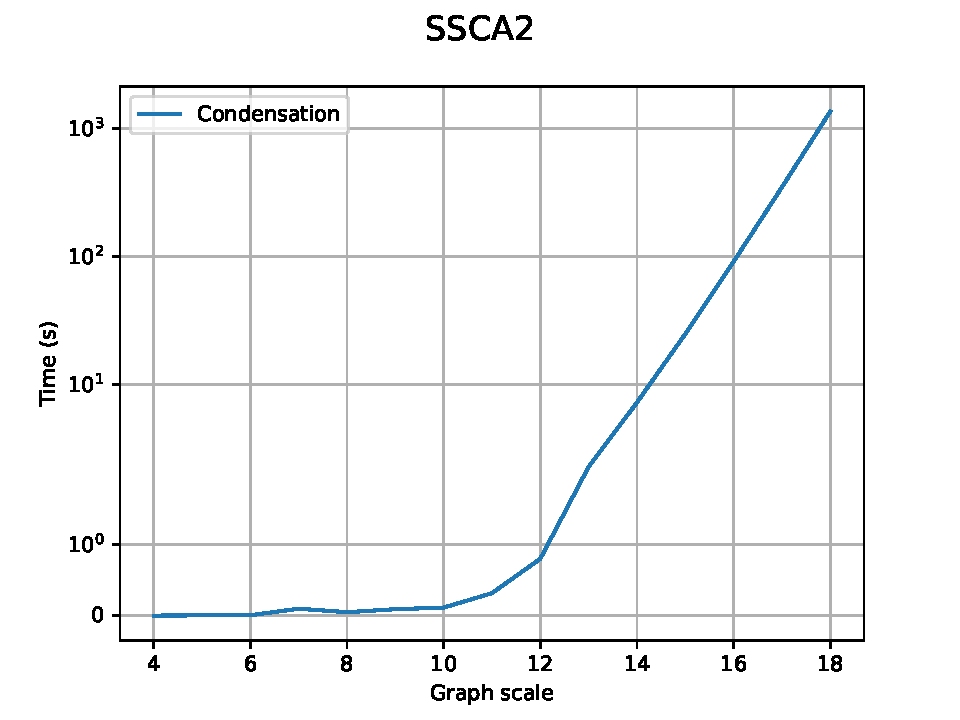
\includegraphics[width=8cm]{images/condensation_SSCA2.pdf}
      \caption{SSCA2}
      \label{fig:condensation:ssca}
    \end{subfigure}
    \begin{subfigure}{.5\textwidth}
      \centering
      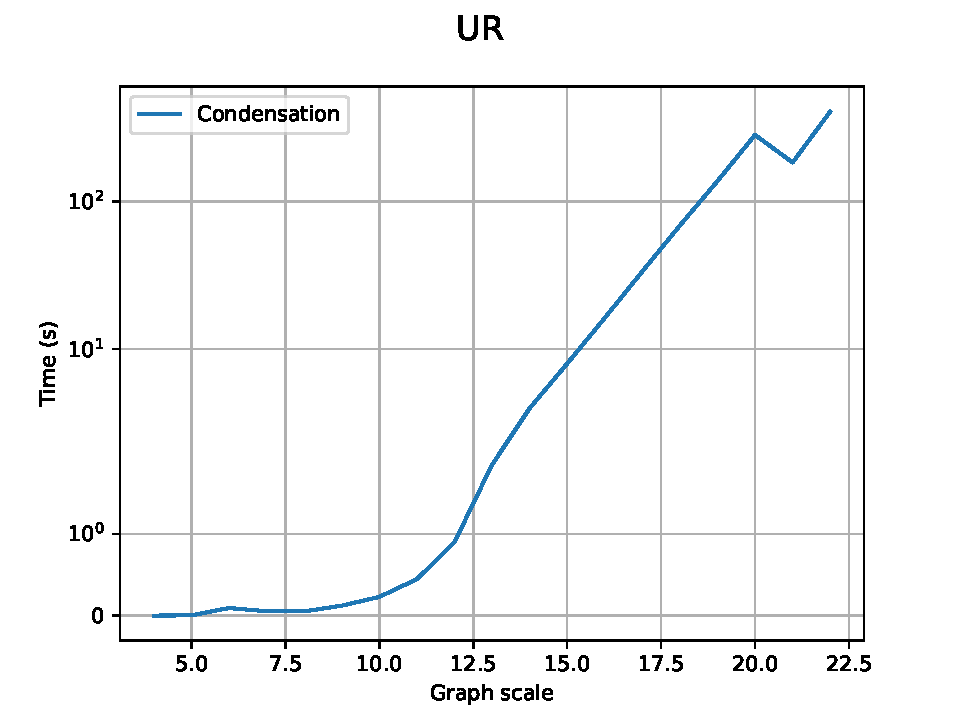
\includegraphics[width=8cm]{images/condensation_UR.pdf}
      \caption{UR}
      \label{fig:condensation:ur}
    \end{subfigure}
    \caption{Зависимость времени конденсации от масштаба графа}
    \label{fig:condensation}
\end{figure}

\FIXME{Что такое масштаб графа в подписи рисунка? Пояснить}

Предобработка занимает $O((N+M)log(M))$. При больших значениях $N, M$ процедура может продолжаться несколько минут.
На рисунке \ref{fig:condensation} показано время работы для различных видов графов.

\begin{table}[H]
  \caption{Влияние конденсации на размер графа}
  \centering
  \begin{tabular}{| c | c | c | c | c |}
  \hline
    & \multicolumn{2}{c |}{До} & \multicolumn{2}{c |}{После} \\ \hline
  Граф & Вершин & Ребер & Вершин & Ребер    \\ \hline
  RMAT & 131072 & 4181810 & 4837 & 4092 \\ \hline
  RMAT & 262144 & 7892410 & 12547 & 10360 \\ \hline
  UR & 131072 & 4193755 & 1 & 0 \\ \hline
  UR & 262144 & 8388074 & 1 & 0 \\ \hline
  SSCA2 & 131072 & 1358656 & 131072 & 1358656 \\ \hline
  SSCA2 & 262144 & 2724762 & 262144 & 2724762 \\ \hline
  \end{tabular}
  \label{table:condensation:impact}
\end{table}

Конденсация дает различные результаты, в зависимости от структуры сжимаемого графа.

Так, Uniform Random графы \cite{erdos1959ur}, как правило состоящие из одной большой КСС, будут сжаты в единственную вершину.
SSCA2 \cite{bader2005ssca} графы почти не имеют компонент сильной связности, поэтому их размер после сжатия в большинстве случаев не изменится.
RMAT \cite{chakrabarti2004rmat} графы уменьшатся в размерах за счет наличия крупных КСС. Сравнение приведено в таблице \ref{table:condensation:impact}

\subsection{Подход к перебору черных дыр}

После предобработки графа происходит переход к этапу поиска черных дыр. Решаемая задача имеет комбинаторную природу, поэтому на данном этапе будет полезно уменьшить число потенциальных кандидатов. Опишем сначала подход к организации полного перебора, который учитывает особенности строения черных дыр.

\begin{definition}\label{def:blackholeroot}
Корень черной дыры $B \subseteq V$ --- это такая вершина $v \in B$, что не найдется ребра $(u, v) \in E$, где $u \in B,\ u \neq v$.
\end{definition}

\begin{definition}\label{def:blackholebasis}
Множество всех корней черной дыры называется базисом черной дыры.
\end{definition}

Отметим, что базис черной дыры может состоять из произвольного числа вершин, отличного от нуля.

\linespread{1.0}
\begin{figure}[H]
	\begin{center}
		\begin{algorithm}[H]
			\SetAlgoLined
			\SetKwInOut{Input}{Input}
			\SetKwInOut{Output}{Output}
			\Input{$G(v, E)$ -- ориентированный граф, $V$ -- множество вершин, $E$ -- множество ребер, \\
                   $n$ -- максимальное число вершин, которое может содержать черная дыра}
			\Output{$Blackholes$ -- множество всех черных дыр графа размером от 1 до n}

                        $Blackholes = \emptyset$ \\
                        \For{$i = 1\ to\ n$} {
                            \ForEach{$C \in V(i)$} {
                                $B = \bigcup\limits_{v \in C} Closure(v)$ \\
                                \If{$G(B)$ -- слабо связан} {
                                    $Blackholes = Blackholes \cup B$
                                }
                            }
                        }
                        \Return $Blackholes$
			\label{alg:basisbruteforce}
			\caption{BasisBruteForce}
		\end{algorithm}
	\end{center}
\end{figure}
\linespread{1.5}

Алгоритм \ref{alg:basisbruteforce} BasisBruteForce показывает, как можно организовать перебор, основываясь на предыдущих утверждениях.
Во время полного перебора просматриваются все возможные неупорядоченные подмножества вершин графа.
Сначала размера 1, потом 2 и так далее.
Далее для каждой вершины очередного подмножества строится ее замыкание.
Объединение всех таких замыканий является потенциальной черной дырой.
Если кандидат является слабо связным подграфом, тогда это черная дыра.
На рисунке \ref{fig:blackholerootscolored} проиллюстрированы описанные действия.

 \FIXME{В подписи рисунка 2 в конце -- точка. В других подписях ее нет. Нужно сделать везде одинаково. Мне больше нравится с точкой в конце}
 
\begin{figure}[H]
      \centering
      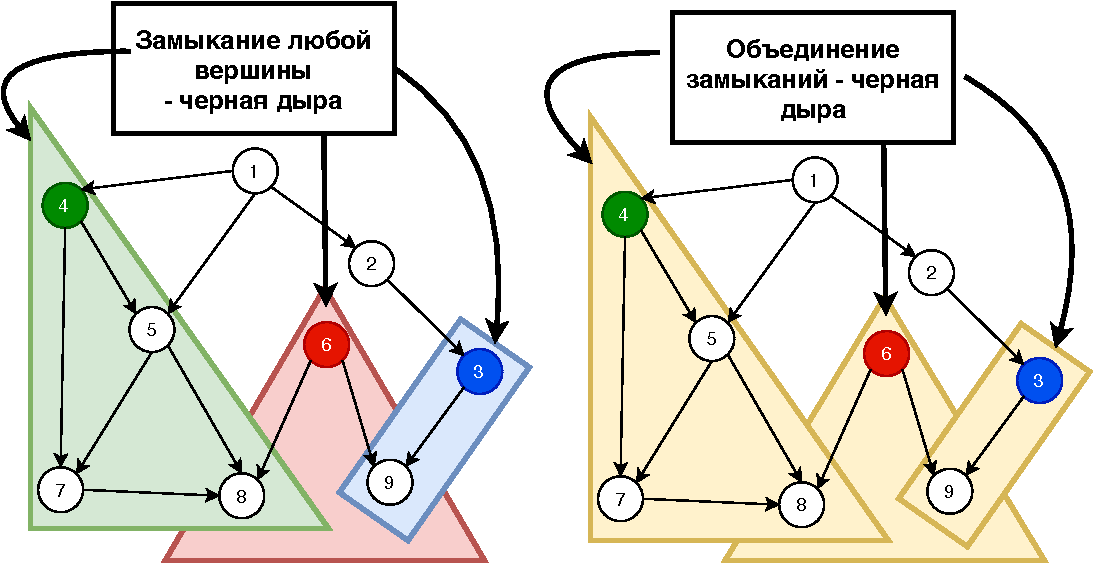
\includegraphics[width=0.8\linewidth]{images/blackhole_roots.pdf}
      \caption{Построение черной дыры по множеству ее корней.
Слева три черных дыры имеющих по одному корню. Справа одна черная дыра с тремя корнями.}
      \label{fig:blackholerootscolored}
\end{figure}

\FIXME{Напрашиваеся -- неформально, переформулировать}
Напрашивается сравнение с алгоритмом \ref{alg:bruteforce} BruteForce.
Отметим, что в описанном варианте перебора отсутствует необходимость проверять число исходящих ребер для периферических вершин. \FIXME{Сокращения (т.к.) недопустимы - по всему тексту лучше проверить}
Т.к по определению замыкания, оно уже содержит все достижимые вершины, то точно известно, что больше не найдется ни одного
исходящего ребра.
К сожалению, такой подход не застрахован от повторного обнаружения уже известной черной дыры.
Для уменьшения количества повторных обнаружений уже известных дыр предлагается
использовать информацию о топологии графа.

\subsection{Сокращение перебора при помощи анализа топологии графа}

Согласно определениям, данным выше, если какая-то вершина не является корнем рассматриваемой черной дыры,
то она может быть опущена, так как набор корней описывает черную дыру единственным образом.
Каждая не корневая вершина в черной дыре достижима из какого-то корня черной дыры.
Значит, при наличии матрицы попарной достижимости для данного графа,
можно эффективно определять лишние, не являющиеся базисами, комбинации вершин.
Конечно же, возникает желание сразу же вычислить такую матрицу достижимости,
но это вычислительно сложная задача $O(V^3)$.
Кроме того, хранение матрицы смежности может потребовать $O(|V|^2)$ памяти, что значительно ограничит применимость такого метода.
Наконец, отметим, что если дан набор вершин размера $K$, то в худшем случае потребуется $K^2/2$ обращений к матрице.
Таким образом, прямое вычисление матрицы достижимости не выглядит разумным решением.
Это может привести к нехватки как памяти, так и времени  на предобработку.
\FIXME{Неплохо бы получить -- неформально, переформулировать}
Надо отметить, что неплохо бы получить первые черные дыры как можно скорее после старта,
что накладывает ограничения на использование особенно дорогих вычислений.

Поэтому вводится правило, которое является частным случаем описанного в предыдущем абзаце,
чтобы частично сократить поле перебора, не жертвуя при этом временем ответа.
Те дубликаты, которые не могут быть отфильтрованы при помощи топологии, будут проверены напрямую.

\begin{definition}
Топологоческая сортировка или топологическое упорядочивание ациклического орграфа --- такой массив вершин, что для любого ребра $(u,v) \in E$ вершина $v$ будет иметь индекс меньше, чем $u$.
\end{definition}

\begin{definition}\label{def:specialnode}
Пусть дан ориентированный граф $G(V,E)$, корень $r \in Roots(G)$, $topSortOrder_r$ ---
топологическая сортировка замыкания $Closure(r)$ и $|Closure(v)|$ ---
размеры замыканий для всех вершин $v \in Closure(r)$, то есть доступных из $r$.
Вершина называется особой вершиной под корнем $r$, если размер ее замыкания $|Closure(v)|$ равен ее индексу в массиве $topSortOrder_r$ плюс один.
\end{definition}

\begin{remark}
Заметим, что множество $Special_r$ особых вершин под корнем $r$ полностью содержится в замыкании данного корня, то есть $Special_r \subseteq Closure(r)$
\end{remark}

\begin{figure}[H]
      \centering
      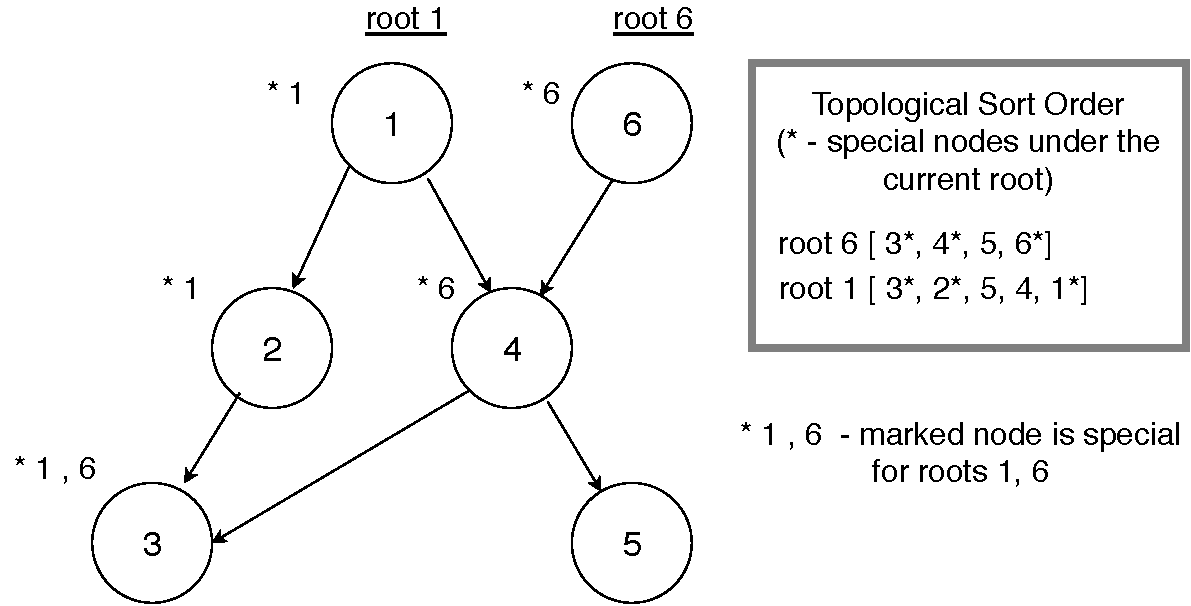
\includegraphics[width=0.8\linewidth]{images/special_nodes.pdf}
      \caption{Граф с двумя корнями (вершины 1 и 6), топологическая сортировка замыканий каждого из корней, особые вершины под каждым корнем отмечены знаком * и номером соответствующего корня.}
      \label{fig:specialnodes}
\end{figure}

\begin{remark}
Решение о том, является ли вершина особой,
принимается независимо в поддереве каждого корня.
Одна и та же вершина может быть особой в поддереве одного корня
и не являться таковой в поддереве другого корня. Пример такой ситуации отображен на рисунке \ref{fig:specialnodes}.
\end{remark}

\begin{definition}
Пусть дан ориентированный граф $G(V,E)$, один из его корней $r \in Roots(G)$,
$topSortOrder_r$ --- топологическая сортировка замыкания $Closure(r)$, $v \in Special_r$ и $u \in Closure(r)$.
Вершина $v$ доминирует над вершиной $u$ под корнем $r$, если $v$ имеет больший индекс, чем $u$ в массиве $topSortOrder_r$.
\end{definition}

\begin{remark}
Если дано две особых вершины под одним корнем, то одна из них всегда будет доминировать над другой.
\end{remark}

\begin{theorem}
Пусть дан ориентированный граф $G(V,E)$, один из его корней $r \in Roots(G)$,
$v \in Special_r$, $u \in Closure(r)$. Если $v$ доминирует над $u$ под корнем $r$, значит $u$ достижима из $v$.
\end{theorem}

\begin{proof}
По определению особой вершины размер замыкания $v$ равен ее индексу плюс один в $topSortOrder_r$.
Рассмотрим все вершины, отличные от $v$ в замыкании $Closure(v)$.
Эти вершины в массиве $topSortOrder_r$ имеют индексы меньше, чем вершина $v$.
Отсюда $\forall u \in Closure(v)$ вершины $u$ будет достижима из $v$.
\end{proof}

\begin{theorem}
Пусть дан ориентированный граф $G(V,E)$, один из его корней $r \in Roots(G)$,
$v \in Special_r$, $u \in Closure(r)$.
Если $v$ доминирует над $u$ под корнем $r$, значит $Closure(v) \cup Closure(u) = Closure(v)$.
\end{theorem}

\begin{proof}
Согласно предыдущей теореме, если $v$ доминирует над $u$ под корнем $r$,
то вершина $u$ будет достижима из $v$.
Тогда $u \in Closure(v)$ откуда следует $Closure(u) \subseteq Closure(v)$.
\end{proof}

\begin{definition}
Те вершины графа $G(V,E)$, которые не имеют входящих ребер, называются глобальными корнями.
\end{definition}

Рассмотрим две вершины в замыкании глобального корня.
Пусть одна из них особая, а другая нет.
Чтобы эти две вершины образовали базис, особая вершина не должна доминировать над обычной.
В противном случае обычная вершина могла бы быть опущена как незначимая.
В общем случае, если дан набор вершин, можно убрать из набора все доминируемые вершины и получить корректный базис.

На рисунке \ref{fig:candidatesfiltering} приведены примеры наборов из двух вершин, не образующих корректный базис
или не удовлетворяющих условию слабой связности.

\begin{figure}[H]
      \centering
      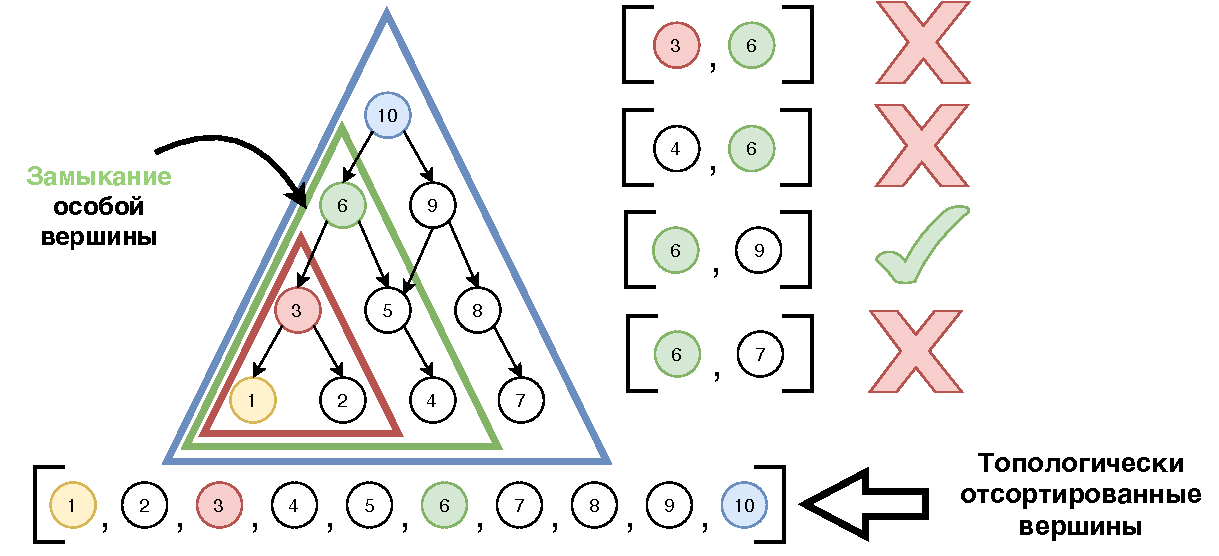
\includegraphics[width=1.0\linewidth]{images/candidates_filtering.pdf}
      \caption{Граф из 10 вершин с единственным корнем и его топологическая сортировка. Цветом выделены особые вершины.
Цветные треугольники обозначают замыкание соответветствующих особых вершин. В правой части приведены примеры наборов кандидатов размера 2.}
      \label{fig:candidatesfiltering}
\end{figure}

\subsection{Алгоритм IsBasis}\label{subsec:isbasis}

Алгоритм \ref{alg:isbasis} (IsBasis)  проверяет, является ли набор вершин базисом.
Этот алгоритм принимает набор вершин и возвращает True, если данный набор образует базис и False в противном случае.
Он используется как составная часть алгоритма TopSortBH, который будет описан позднее.

IsBasis действует следующим образом.

В первую очередь нам нужно знать, какие вершины являются особыми.
Этот шаг может быть посчитан заранее. Чтобы определить особые вершины,
построим топологическую сортировку замыкания для каждого глобального корня.
Далее по определению \ref{def:specialnode} отметим особые вершины.

Вторым шагом, если хотя бы одна из вершин набора доминируема, то данный набор вершин пропускается.

На третьем шаге закончились дешевые методы принятия решения.
Проверяем попарную достижимость вершин в наборе.
Если найдется хоть одна такая пара, опускаем данный набор вершин.

Если ни одна из предыдущих проверок не ответила False (Пропустить), то алгоритм IsBasis возвращает True.
Это значение возвращается в алгоритм TopSort и означает, что текущий набор вершины является корректным базисом черной дыры.
Здесь есть небольшая оговорка. Проверки, которые проводит IsBasis никак не учитывают слабую связность
графа, индуцированного рассматриваемым набором вершин.

\linespread{0.93}
\begin{figure}[H]
	\begin{center}
		\begin{algorithm}[H]
			\SetAlgoLined
			\SetKwInOut{Input}{Input}
			\SetKwInOut{Output}{Output}
			\Input{$G(V,E)$ -- ориентированный граф без циклов (граф конденсация) \\
                                $Cand \subset V$ -- множество вершин, потенциальный базис черной дыры}
			\Output{$True$ -- если $Cand$ является базисом черной дыры, $False$ в противном случае}
                        \tcc{(1) определить особые вершины для каждого корня}
                        \ForEach{$r \in Roots(G)$} {
                            $Special_r = \emptyset$ \\
                            $build\ topSortOrder_r$ \\
                            \For{$i = 0; i<|topSortOrder_r|; i=i + 1$} {
                                $v = topSortOrder_r[i]$ \\
                                $C_v = Closure(v)$ \\
                                \If{$|C_v| == i$} {
                                    $Special_r = Special_r \cup v$ \\
                                    $maxSpecialIndex_r = max(maxSpecialIndex_r, i)$ \\
                                }
                            }
                        }
			\tcc{(2) проверить, есть ли доминируемые вершины}
                        \ForEach{$r \in Roots(G)$} {
                            $maxSpecialIndex_r = -1$ \\
                        }
			\ForEach{$v \in Cand$} {
                            \ForEach{$r \in Roots(G)$} {
                                \If{$v \in Special_r$} {
                                    $vTopSortIndex_r = arg_v (topSortOrder_r)$ \\
                                    $maxSpecialIndex_r = max(maxSpecialIndex_r, vTopSortIndex_r)$ \\
                                }
                            }
			}
			\ForEach{$v \in Cand$} {
                            \ForEach{$r \in Roots(G)$} {
                                \If{$v \in Closure(r)$} {
                                    $vTopSortIndex_r = arg_v (topSortOrder_r)$ \\
                                    \If{$vTopSortIndex_r < maxSpecialIndex_r$} {
                                        \Return $False$ \\
                                    }
                                }
                            }
			}
                        \tcc{(3) проверить вершины на взаимную достижимость}
                        \ForEach{$(v, u) \in Cand(G) \times Cand(G)$} {
                            \If{v is reachable from u} {
                                \Return $False$ \\
                            }
                        }
                        \Return $True$
			\label{alg:isbasis}
			\caption{IsBasis}
		\end{algorithm}
	\end{center}
\end{figure}
\linespread{1.5}


\subsection{Алгоритм TopSortBH}\label{subsec:topsortbh}

\linespread{1.0}
\begin{figure}[H]
	\begin{center}
		\begin{algorithm}[H]
			\SetAlgoLined
			\SetKwInOut{Input}{Input}
			\SetKwInOut{Output}{Output}
			\Input{$G(V,E)$ -- ориентированный граф}
			\Output{$Blackholes$ -- множество черных дыр разных размеров}

                        $Blackhole = \emptyset$\\
                        Построить граф конденсацию $Cond(V',E')$ \\
                        \For{$i = 1\ to\ |V'|$} {
                            $cnt_i = 0$ \\
                            \ForEach{$B_i \in V'(i)$} {
                                \If{$IsBasis(Cond(V',E'),B_i)$} {
                                    \If{$B_i$ -- слабо связан} {
                                        $Blackholes = Blackholes \cup B_i$ \\
                                        $cnt_i = cnt_i + 1$
                                    }
                                }
                            }
                            \If{$cnt_i == 0$} {
                                \Return $Blackholes$
                            }
                        }
                        \Return $Blackholes$
			\label{alg:topsort}
			\caption{TopSortBH}
		\end{algorithm}
	\end{center}
\end{figure}
\linespread{1.5}

Предлагаемый нами алгоритм \ref{alg:topsort} TopSortBH является комбинацией трех составных частей, которые были описаны ранее.
    \begin{itemize}
        \item Предобработка: конденсация графа;
        \item Перебор черных дыр при помощи алгоритма \ref{alg:basisbruteforce} BasisBruteForce;
        \item Сокращение перебора при помощи алгоритма \ref{alg:isbasis} IsBasis на основе информации о топологии графа.
    \end{itemize}

Данный алгоритм действует следующим образом.

Для входного графа строится его конденсация.
Далее под графом всегда понимаем именно сконденсированный вариант.

Перебираются наборы вершин размером от $1$ до $N$, и проверяются алгоритмом IsBasis.
Если для некоторого набора возвращается $False$, то такой набор сразу же пропускается.
Если для некоторого набора возвращается $True$, то для получения черной дыры,
необходимо, согласно определению, объединить все замыкания его вершин.
Последний шаг заключается в проверке полученного множество на слабую связность.
Если данное свойство присутствует, то это будет означать, что получена черная дыра.

Если не было найдено ни одного корректного базиса размера $K$, это значит, что
не найдется ни одного корректного базиса размером $K + 1$. А значит, в такой ситуации
можно остановить перебор.

\FIXME{Или от iBlackholeDC?}

Отметим основные отличия данного алгоритма от iBlackhole:
    \begin{itemize}
        \item Перебираются не наборы вершин, а наборы корней;
        \item Любой набор, даже тот, что не прошел проверку IsBasis, на самом деле образует черную дыру, если удовлетворяет требованию слабой связности.  Для iBlackhole такого условия будет недостаточно.
        \item Нельзя задать конкретный размер черной дыры для поиска. Для этого потребовалось бы хранить информацию о размерах замыканий вершин и их пересечений;
        \item Отсутствует связь между итерациями. Для каждого отдельно взятого набора решение принимается независимо;
        \item Если в графе отсутствуют черные дыры определенных размеров, то это не скажется на работе алгоритма TopSortBH. Он будет перебирать только те черные дыры, которые фактически присутствуют.
    \end{itemize}

\subsection{Гибридный алгоритм TopOver}\label{subsec:topover}

Предложенный выше алгоритм TopSortBH не позволяет ограничить размер рассматриваемых черных дыр.
Такая возможность есть у алгоритма iBlackholeDC. Его процесс отбора вершин-кандидатов устроен таким
образом, что если провести единственную итерацию при $i=K$, то останется множество вершин,
которые могут образовывать черные дыры размером не больше, чем $K$. Когда такое множество
вершин получено, необходимо перебрать наборы вершин и проверить на соответствие
определению черной дыры.

\linespread{1.0}
\begin{figure}[H]
	\begin{center}
		\begin{algorithm}[H]
			\SetAlgoLined
			\SetKwInOut{Input}{Input}
			\SetKwInOut{Output}{Output}
			\Input{$G(v, E)$ -- ориентированный граф, $V$ -- множество вершин, $E$ -- множество ребер, \\
                   $n$ -- максимальное число вершин, которое может содержать черная дыра}
			\Output{$Blackholes$ -- множество всех черных дыр графа размером от 1 до n}
                        Построить граф конденсацию $GC = Cond(V',E')$ \\
                        $Blackholes = \emptyset$ \\
                        $P_n = \{v | d_{out}(v) < n\}$ \\
                        убрать лишние вершины из $P_n$ и сформировать список кандидатов $C_n$ \\
                        убрать лишние вершины из $C_n$ и сформировать список кандидатов $F_n$ \\
                        \ForEach{$WCC \in GC(F_n)$} {
                            \tcc{Применить алгоритм TopSortBH к $GC(WCC)$}
                            $Blackholes = Blackholes \cup TopSortBH(GC(WCC))$
                        }
                        \Return $Blackholes$
			\label{alg:topover}
			\caption{TopOver}
		\end{algorithm}
	\end{center}
\end{figure}
\linespread{1.5}

Воспользуемся отбором кандидатов на основе iBlackholeDC, а в качестве алгоритма перебора используем TopSortBH.
Таким образом, получим алгоритм-комбинацию \ref{alg:topover} TopSortBH over iBlackholeDC (TopOver).
Заметим, что в данном случае конденсация графа производится один раз до начала отбора кандидатов.
Так как на вход TopSortBH передается уже сконденсированный граф, то повторная конденсация не требуется.
Размеры исходных КСС не учитываются при определении размера черной дыры. При возникновении такой необходимости
алгоритм легко модифицировать.

\subsection{Аспекты параллелизма в рассмотренных алгоритмах}\label{subsec:parallelresource}

Все представленные алгоритмы обладают запасом параллелизма.
Рассмотрим подробнее алгоритмы \ref{alg:iblackholedc} iBlackholeDC и \ref{alg:topsort} TopSortBH.
Первый из них обладает параллелизмом на четырех уровнях:

1. Параллелизм итераций. Здесь, как уже упоминалось, есть оговорка.
\FIXME{Просто замечание, что в исходном алгоритме нет зависимости по итерациям, все итерации независимы. Поэтому я не согласен, что итерации связаны.}
Строго говоря, каждая итерация обращается к результатам предыдущей.
Таким образом, в алгоритме удается избежать повторного принятия решений о тех вершинах,
которые ранее уже были добавлены во множество кандидатов.
Эту проверку можно проигнорировать и начать вычисления с любой итерации.
Тогда множество ранее утвержденных кандидатов окажется пусто, и для
каждой вершины придется принимать решение. Результат будет верен в любом случае.
Значит, каждую итерацию (или последовательность итераций) можно запустить на отдельном вычислителе.
Эффективнее распределять итерации блоками, это сократит накладные расходы.

2. Параллелизм рассмотрения кандидатов. Решение о добавлении очередной вершины
в множество кандидатов можно принимать независимо от остальных внутри итерации.
В этом случае важно, чтобы множество кандидатов с предыдущей итерации было полностью сформировано.

3. Параллелизм компонент слабой связности. Каждую компоненту слабой связности графа, индуцированного
набором кандидатов, можно рассматривать независимо.

4. Параллелизм перебора. Работу по перебору подмножеств кандидатов можно распределить между узлами.
Для этого достаточно пронумеровать все наборы. \FIXME{а почему нельзя динамически распределить нагрузку в зависимости от кол-ва кандидатов? В момент передачи управления на этот цикл кол-во итераций известно}


Теперь о параллелизме алгоритма TopSortBH.

1. Параллелизм компонент слабой связности. Исходный граф можно разделить на копоненты слабой связности
и каждую обрабатывать независимо.

2. Параллелизм перебора. Здесь можно выделить два подуровня параллелизма.

2а. Параллелизм размеров множеств-кандидатов. Каждый размер можно рассматривать независимо.
Между размерами нет связи по данным (в отличие от итераций iBlackholeDC), что дает значительный простор
для параллельной обработки.
В рамках одного размера удобно применять эвристики для сокращения перебора на основе топологии.

2б. Параллелизм перебора. Для каждого выбранного размера подмножества существует большое количество
комбинаций выбора. Для каждой такой комбинации решение принимается независимо.

\subsection{Детали реализации}\label{subsec:implementation}

В этом разделе рассмотрим несколько особенностей реализации алгоритма TopSortBH.

Все описанные алгоритмы реализованы на языке С++. Для написания параллельного кода
над общей памятью использовалась технология OpenMP.

\subsubsection{О работе с графом}\label{subsubsec:graph}

Граф хранится в виде списков смежности. То есть для каждой вершины хранится список номеров вершин,
в направлении которых есть ориентированные ребра. Все графы считаются ориентированными.
В неориентированном графе для каждого ребра существует обратное ему по направлению. Такой подход
позволяет использовать одинаковые реализации алгоритмов как для ориентированных,
так и для неориентированных графов.

Кроме исходного графа для работы алгоритмов часто требуются граф с инвертированными ребрами и неориентированный граф.
Так, например, в iBlackholeDC возникает задача построения замыкания вершины по обратным ребрам.
Проверку слабой связности удобно реализовать обходом вершин в неориентированном графе.
Поэтому алгоритмы на ранних стадиях работы строят инвертированный и неориентированный графы.

%\subsubsection{Ввод-вывод}\label{subsubsec:graph}
%
%Граф хранится в бинарном файле. В начале записано два числа:
%количество вершин и количество ребер графа. Далее следуют пары номеров вершин,
%каждая из которых соответствует ориентированному ребру.
%
%Для вывода результатов используется текстовый файл.

\subsubsection{Проверка слабой связности}\label{subsubsec:connectivitycheck}

Для проверки слабой связности используется обход в ширину на неориентированном графе.

\begin{lstlisting}[language=C++, caption=Проверка слабой связности множества корней, label=code:connectivity]
bool CheckConnectivity(const TGraph& graphUndir,
                       const set<size_t>& bh)
{
    TUsed used;
    used.assign(graphUndir.size(), 1);
    for (size_t v : bh) {
        used[v] = 0;
    }
    size_t v = *bh.begin();
    TClosure closure = GetClosure(graphUndir, v, used);
    return closure.size() == bh.size();
}
\end{lstlisting}

Создается массив used, в котором 0 помечаются вершины из проверяемого множества.
От произвольной вершины запускается процедура обхода замыкания вершины.
Обход посещает только те вершины, которые отмечены 0, а уже обойденные
помечает 1.
Если размер замыкания совпадает с размером проверяемого множества, значит,
присутствует слабая связность. Код приведен в листинге \ref{code:connectivity}.

\subsubsection{Проверка попарной достижимости}\label{subsubsec:reachabilitycheck}

Проверка попарной достижимости корней встроена в функцию GetBlackhole.
Ee код представлен в листинге \ref{code:reachability}.
GetBlackhole для заданного графа $graph$, топологической сортировки $tsOrder$ и набора позиций в нем
строит множество вершин черной дыры. Если среди корней находится хотя бы одна доминируемая вершина,
то будет возвращено пустое множество.

Массив $used$ содержит в себе счетчики количества посещений для каждой вершины графа.
При обходе очередного замыкания (см. Листинг \ref{code:getclosure}), все вершины, которые
были посещены или хотя бы рассмотрены к посещению, увеличивают свои счетчики на 1.
Если одна из вершин может быть достигнута различными путями от одного корня,
то ее счетчик может быть увеличен только единожды. Если корень может быть достигнут
при обходе замыкания другого корня, то его счетчик после обхода всех корней станет больше или равен 2.
Если это так, то такая черная дыра могла быть обнаружена при просмотре кандидатов меньшего размера,
а значит должна быть пропущена.

Важно заметить, что такой алгоритм проверки будет работать только на сконденсированном графе.

\begin{lstlisting}[language=C++, caption=Построение черной дыры по набору корней, label=code:reachability]
set<size_t> GetBlackHole(const TGraph& graph,
                         const vector<size_t>& tsOrder,
                         const vector<size_t>& pos)
{
    set<size_t> blackhole;
    TUsed used;
    used.assign(graph.size(), 0);
    for (size_t p : pos) {
        size_t v = tsOrder[p];
        TClosure closure = GetClosure(graph, v, used);
        for (size_t x : closure) {
            blackhole.insert(x);
        }
    }
    for (size_t p : pos) {
        size_t x = tsOrder[p];
        if (used[x] >= 2) {
            return {};
        }
    }
    return blackhole;
}
\end{lstlisting}

\begin{lstlisting}[language=C++, caption=Обход замыкания данной вершины, label=code:getclosure]
TClosure GetClosure(const TGraph& g, size_t v, TUsed& used) {
    return ClosureBFS(g, used, v);
}

TClosure ClosureBFS(const TGraph& g,
                    TUsed& used, size_t s)
{
    TUsed localUsed(used.size(), 0);
    queue<size_t> q;
    TClosure closure;
    if (!used[s]) {
        q.push(s);
        closure.insert(s);
    }
    used[s] += 1;
    localUsed[s] += 1;
    while(!q.empty()) {
        size_t v = q.front();
        q.pop();
        for (size_t to : g[v]) {
            if (!localUsed[to]) {
                if (!used[to]) {
                    q.push(to);
                    closure.insert(to);
                }
                used[to] += 1;
                localUsed[to] += 1;
            }
        }
    }
    return closure;
}
\end{lstlisting}

\subsubsection{Сокращение перебора}\label{subsubsec:shouldskip}

Как было описано выше, наличие доминируемых вершин в наборе корней,
позволяет пропустить этот набор, так как его можно свести к другому,
меньшего размера. Чтобы понять, что в наборе есть хотя бы одна
доминируемая вершина, не проверяя достижимости,
необходимо убедиться, что не найдется особой вершины,
которая была бы топологически выше другой вершины в наборе.

Функция ShouldSkip (Листинг \ref{code:shouldskip}) осуществляет такую проверку.
Массив $pos$, как и ранее, содержит в себе упорядоченные по
возрастанию номера позиций корней черной дыры в массиве tsOrder.
Массив tsOrder содержит порядок топологической сортировки графа.
Правило, описанное выше, эквивалетно тому, что особая вершина может быть
самой низкой в топологии набора и при этом единственной.
Таким образом, как только обнаружена особая вершина на любой
позиции, начиная со второй, можно делать вывод, что набор не подходит.

\begin{lstlisting}[language=C++, caption=Проверка множества на наличие доминируемых вершин, label=code:shouldskip]
bool ShouldSkip(const vector<size_t>& tsOrder,
                const vector<char>& special,
                const vector<size_t>& pos)
{
    for (size_t i = 1; i < pos.size(); i++) {
        size_t p = pos[i];
        size_t v = tsOrder[p];
        if (special[v]) {
            return true;
        }
    }
    return false;
}
\end{lstlisting}

\subsection{Модификация Skip Precise}\label{subsec:preciseskip}

\begin{lstlisting}[language=C++, caption=Пропуск сразу нескольких наборов кандидатов без ложно-отрицательных результатов, label=code:preciseskip]
void ForceSkipPrecise(const vector<size_t>& tsOrder, const vector<char>& special, std::vector<size_t>& pos) {
    size_t skip = 0;
    for (size_t i = 1; i < pos.size(); i++) {
        size_t p = pos[i];
        size_t v = tsOrder[p];
        if (special[v]) {
            skip = i;
            break;
        }
    }
}
\end{lstlisting}
\FIXME{Перенес сюда часть кода, у меня не компилируется}
%	for (size_t i = skip + 1; i < pos.size(); i++) {
%	pos[i] = tsOrder.size() - pos.size() + i;
%}



Пусть дан массив $pos$, который содержит в себе особую вершину на некоторой позиции $skip \neq 0$.
Как было сказано в предыдущем пункте, такой массив $pos$ будет иметь в себе избыточные элементы, а
потому не может являться корректным базисом. Следовательно, его необходимо пропустить.
Если рассмотреть значения на отрезке индексов $[0, skip]$, и рассмотреть массив $[..., skipVal, ....]$ то станет ясно, что любой массив $pos'$
с таким префиксом не будет формировать корректный базис. Таким образом, можно сразу же переходить
к набору $[..., skipVal + 1, skipVal + 2, ..., skipVal + pos.size() - skip]$
тем самым пропуская проверку для всех наборов с рассмотренным префиксом.
Отметим, что для удобства реализации, на самом деле, мы перейдем не к следующему корректному набору
кандидатов, а к последнему набору из некорректной последовательности.
Реализация данного правила представлена в листинге \ref{code:preciseskip}.

\subsection{Модификация Skip Fast}\label{subsec:fastskip}

\begin{lstlisting}[language=C++, caption=Пропуск большого числа кандидатов. Допускаются ложно-отрицательные результаты., label=code:fastskip]
void ForceSkipFast(const vector<size_t>& tsOrder, const vector<char>& special, std::vector<size_t>& pos) {
    size_t skip = 0;
    for (size_t i = 1; i < pos.size(); i++) {
        size_t p = pos[i];
        size_t v = tsOrder[p];
        if (special[v]) {
            skip = i;
            break;
        }
    }

}
\end{lstlisting}

\FIXME{Перенес сюда часть кода, у меня не компилируется}
%    size_t skipPos = pos[skip];
%pos[0] = skipPos - 1;
%for (size_t i = 1; i < pos.size(); i++) {
%	pos[i] = tsOrder.size() - pos.size() + i;
%}


В силу комбинаторной природы задачи, рассмотрение всех черных дыр некоторого графа может
потребовать больших временных ресурсов. В ситуации, когда необходимо быстро обнаружить
как можно больше любых черных дыр, можно прибегнуть к более агрессивной политике сокращения
перебора. Для такого случая можно применить представленную в листинге \ref{code:fastskip}
эвристику.

Пусть дан массив $pos$, который содержит в себе особую вершину на некоторой позиции $skip \neq 0$.
Попробуем сформировать массив $pos'$ такой, что единственная особая вершина, если такая найдется,
будет находиться по индексу равному $0$.
Мы знаем, что особая вершина  находится в позиции $skip$. Перейдем от массива $[..., skipVal, ...]$ к массиву
$[skipVal, skipVal + 1, skipVal + 2, ... , skipVal + pos.size() - skip]$.
Такой набор по построению будет иметь особую вершину на первой позиции, но не обязательно будет являться корректным базисом.

Данный метод приводит к появлению ложно-отрицательных результатов, но значительно увеличивает число обнаруженных за
ограниченное время черных дыр, что отражено в экспериментальной части. В то же время, использование данной эвристики
сокращает число просмотренных, но пропущенных кандидатов.

\cleardoublepage
\section{Результаты экспериментальных исследований}\label{sec:experimentalresults}

Для сравнения разработанных алгоритмов был проведен ряд экспериментов.
Сравнение производилось на трех типах графов RMAT, SSCA2, и UR.
Все запуски были произведены на системе Polus, состоящей из 5 узлов \cite{polus}.
Характеристики узла выглядят следующим образом:
\begin{itemize}
\item 2 десятиядерных процессора IBM POWER8 (каждое ядро имеет 8 потоков), всего 160 потоков
\item Общая оперативная память 256 Гбайт (в узле 5 оперативная память 1024 Гбайт) с ЕСС контролем
\item 2 х 1 ТБ 2.5” 7K RPM SATA HDD
\item 2 x NVIDIA Tesla P100 GPU, 16Gb, NVLink
\item 1 порт 100 ГБ/сек
\item Производительность кластера (Tflop/s): 55,84 (пиковая), 40,39 (Linpack)
\end{itemize}

\subsection{iBlackholeDC vs TopSortBH}\label{subsec:vanillasucks}

В первую очередь было проведено сравнение iBlackholeDC и TopSortBH на графах небольшого размера.
В работе \cite{li2010detecting} алгоритм iBlackholeDC уже испытывался на похожих по размеру графах.
Теперь же было проведено его сравнение с представленным в данной работе TopSortBH.

iBlackholeDC запускался в один поток. Алгоритм был реализован по описанию в оригинальной статье 2010
года и больше не изменялся.
TopSortBH запускался в 8 потоков. Здесь проводится не равное сравнение, поскольку
есть цель подчеркнуть, что представленный в данной работе алгоритм хорошо подходит для параллельной работы, а также
показать общее преимущество достигнутое по результатам работы.
Оба алгоритма получали на вход граф без предобработки. Таким образом, конденсация графа,
которая необходима алгоритму TopSortBH для корректной работы, учитывалась в общем времени его работы.

\FIXME{Пояснить здесь в тексте один раз, что такое Timeout. Далее достаточно использовать это обозначение в подписи к рисунку}

\begin{figure}[H]
    \begin{subfigure}{.5\textwidth}
      \centering
      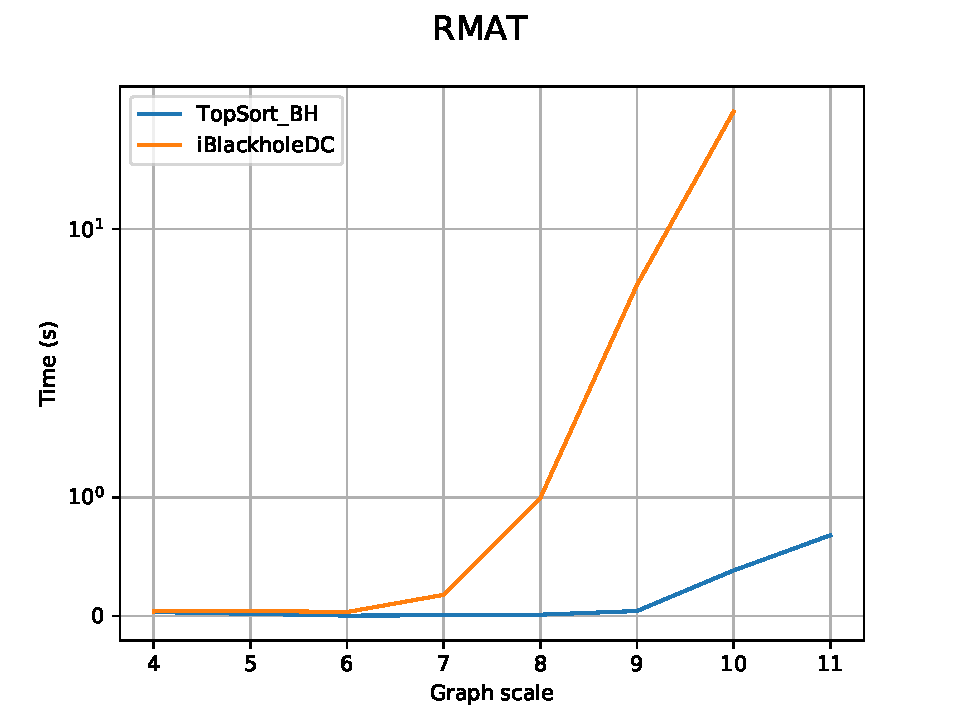
\includegraphics[width=8cm]{images/1_RMAT.pdf}
      \caption{RMAT}
      \label{fig:vanilla:rmat}
    \end{subfigure}
    \begin{subfigure}{.5\textwidth}
      \centering
      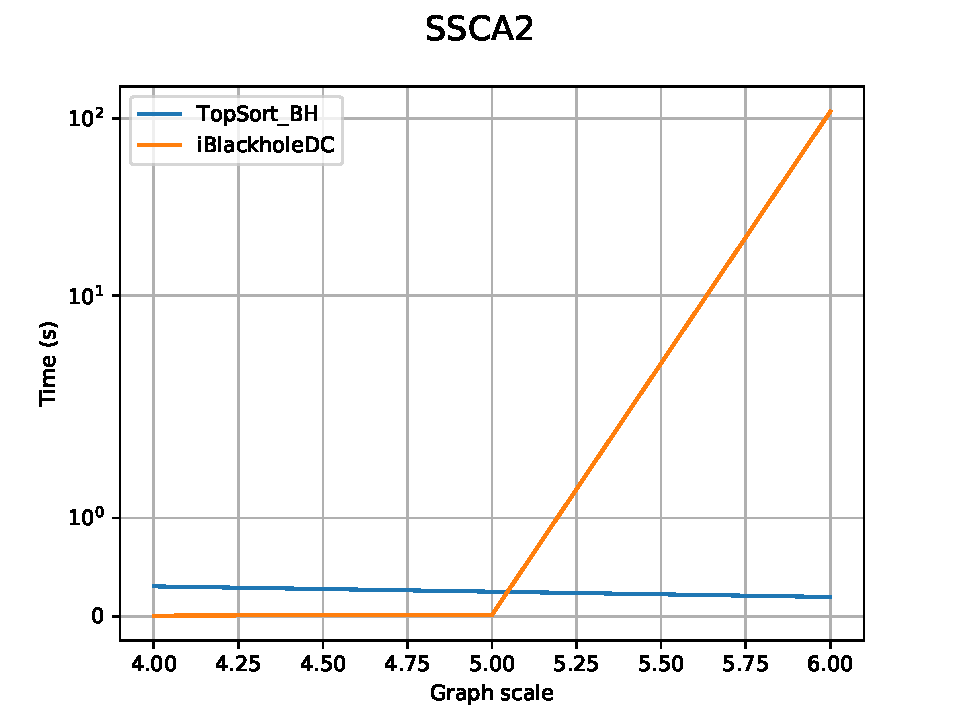
\includegraphics[width=8cm]{images/1_SSCA2.pdf}
      \caption{SSCA2}
      \label{fig:vanilla:ssca}
    \end{subfigure}
    \begin{subfigure}{.5\textwidth}
      \centering
      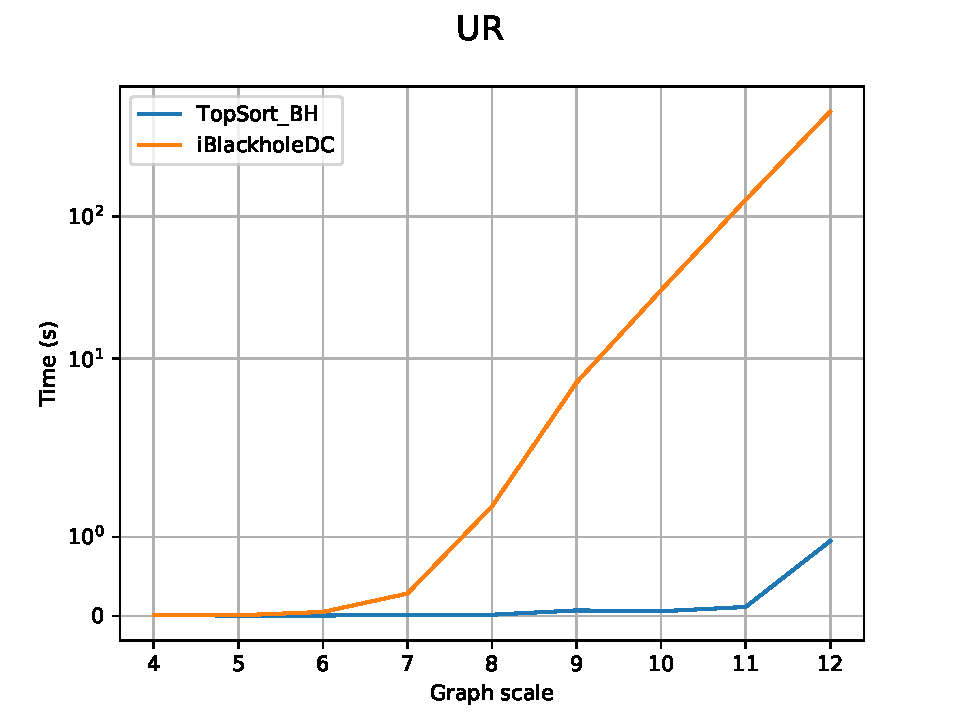
\includegraphics[width=8cm]{images/1_UR.pdf}
      \caption{UR}
      \label{fig:vanilla:ur}
    \end{subfigure}
    \caption{Алгоритм iBlackholeDC, запущенный в 1 потоке, и алгоритм TopSortBH, запущенный с использованием 8 потоков. Установлен Timeout: 30 минут.}
    \label{fig:vanilla}
\end{figure}

На рисунке \ref{fig:vanilla:rmat} показано, что iBlackholeDC не уложился в ограничение по времени для графов масштабом больше 10.
TopSortBH успел отработать на всех графах, кроме масштаба 12, и время его работы не превышало секунды.

На рисунке \ref{fig:vanilla:ssca} видим, что iBlackholeDC показывал преимущество на графах совсем маленьких размеров, но начал проигрывать в последствии.
Оба алгоритма переставали укладываться в отведенное время после масштаба 6 SSCA2 графа. Эти графы хуже всего поддаются любым эвристикам и сжатиям,
в них ярче всего проявляется комбинаторная природа задачи.

В случае графа UR Рис. \ref{fig:vanilla:ur} оба алгоритма уложились в отведенное время для всех представленных размеров, однако TopSortBH был быстрее во всех
случаях. Здесь конденсация графа имеет решающее значение для времени работы алгоритма.

\begin{figure}[H]
    \centering
    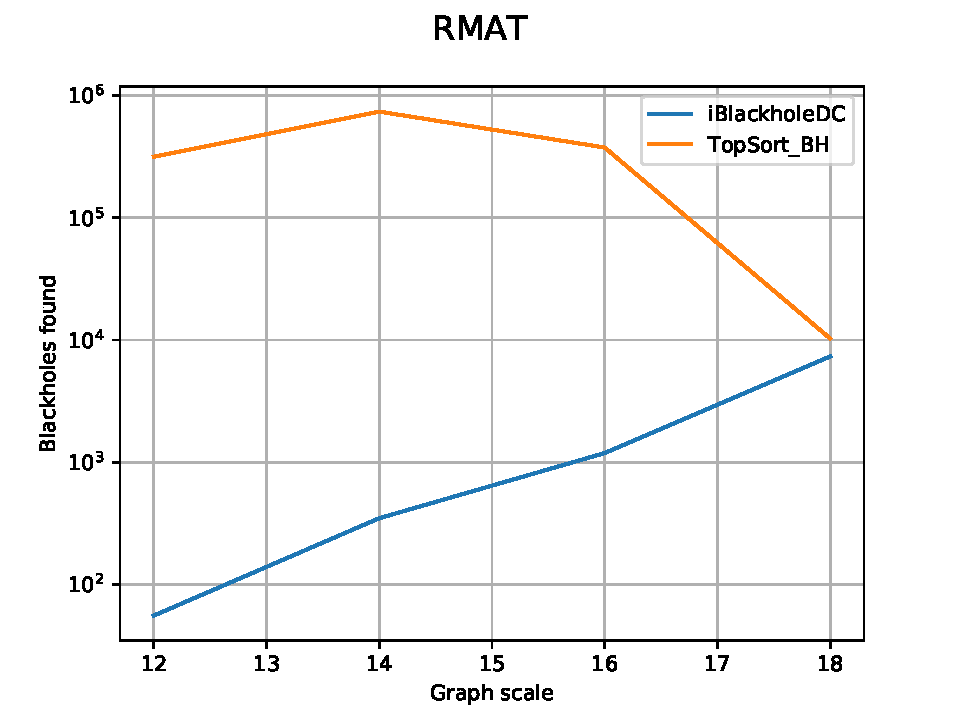
\includegraphics[width=0.8\textwidth]{images/1_large_RMAT.pdf}
    \caption{Алгоритм iBlackholeDC, запущенный в 1 потоке, и алгоритм TopSortBH, запущенный с использованием 8 потоков на графах большого размера.
По оси Y отложено найденное количество черных дыр. Timeout: 3 часа}
    \label{fig:vanillalarge}
\end{figure}

Также было проведено сравнение производительности для RMAT графов больших размеров. Сложность подобного сравнения заключается в том,
что такие графы обрабатываются очень долго и конечный результат может зависеть от структуры графа и заданного ограничения по времени.
На рисунке \ref{fig:vanillalarge} показано количество найденных черных дыр за 3 часа. В правой части графики начинают сходится.
Предположительно, это особенность конкретно взятого графа в сочетании с выбранным временем останова. Последнее может особенно сильно влиять
на показатели алгоритмов относительно друг друга.

\FIXME{не нужно использовать в тексте работе vs, это неформально. Исправьте, пожалуйста, везде}

\subsection{iBlackholeDC vs TopOver}\label{subsec:topovercomparison}

\begin{figure}[H]
    \begin{subfigure}{.5\textwidth}
      \centering
      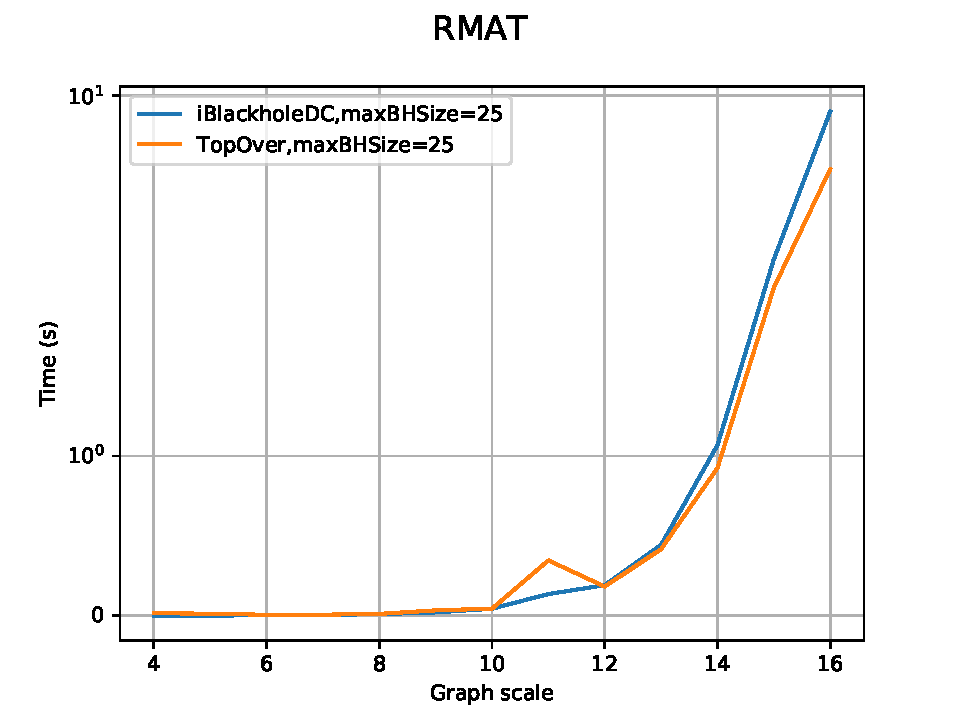
\includegraphics[width=8cm]{images/2_RMAT.pdf}
      \caption{RMAT}
      \label{fig:topochi:rmat}
    \end{subfigure}
    \begin{subfigure}{.5\textwidth}
      \centering
      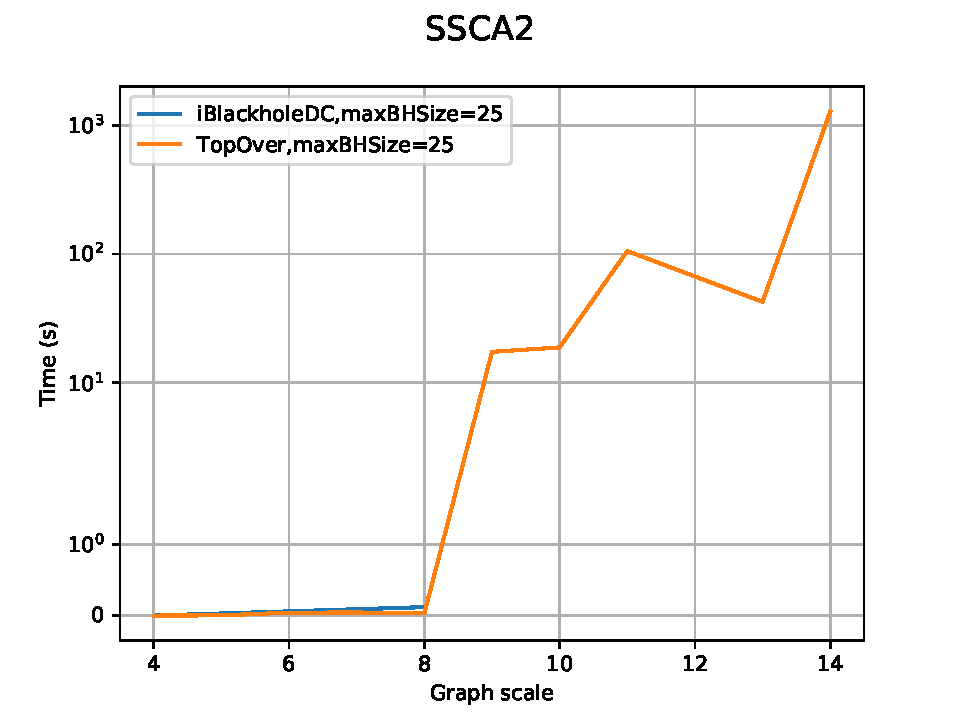
\includegraphics[width=8cm]{images/2_SSCA2.pdf}
      \caption{SSCA2}
      \label{fig:topochi:ssca}
    \end{subfigure}
    \begin{subfigure}{.5\textwidth}
      \centering
      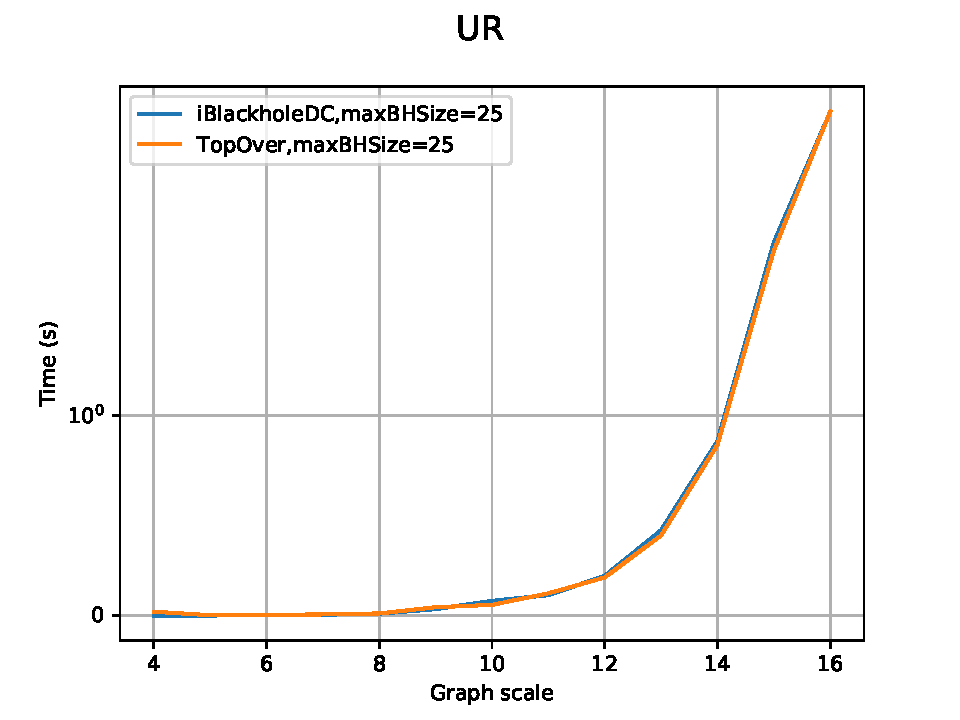
\includegraphics[width=8cm]{images/2_UR.pdf}
      \caption{UR}
      \label{fig:topochi:ur}
    \end{subfigure}
    \caption{Алгоритмы iBlackholeDC и TopOver. Оба запущены с использованием 1 потока. Осуществляется поиск черных дыр размером до 25 вершин. Timeout: 30 минут}
    \label{fig:topochi}
\end{figure}

\FIXME{Может iBlackholeDC в следующем предложении?}

Переходим к сравнению алгоритма TopOver и оригинального iBlackhole.
Эти алгоритмы сравниваем в режиме поиска черных дыр ограниченного размера.
В качестве такого размера было выбрано число 25.
Запуски производились на графах масштабом до 16.
На графах RMAT рис. \ref{fig:topochi:rmat} алгоритмы показывают сравнимую производительность,
однако при увеличении размера графа TopOver алгоритм демонстрирует ярко выраженное преимущество.
В случае UR рис. \ref{fig:topochi:ur} графов разница между алгоритмами отсутствует.
На графах SSCA2 рис. \ref{fig:topochi:ssca} iBlackhole не успевает отработать для масштабов больше 8, а TopOver укладывается
в полчаса на графах масштабом до 14 включительно.

\subsection{Алгоритм iBlackholeDC на сконденсированных графах}\label{subsec:chineseasync}

\begin{figure}[H]
    \begin{subfigure}{.5\textwidth}
      \centering
      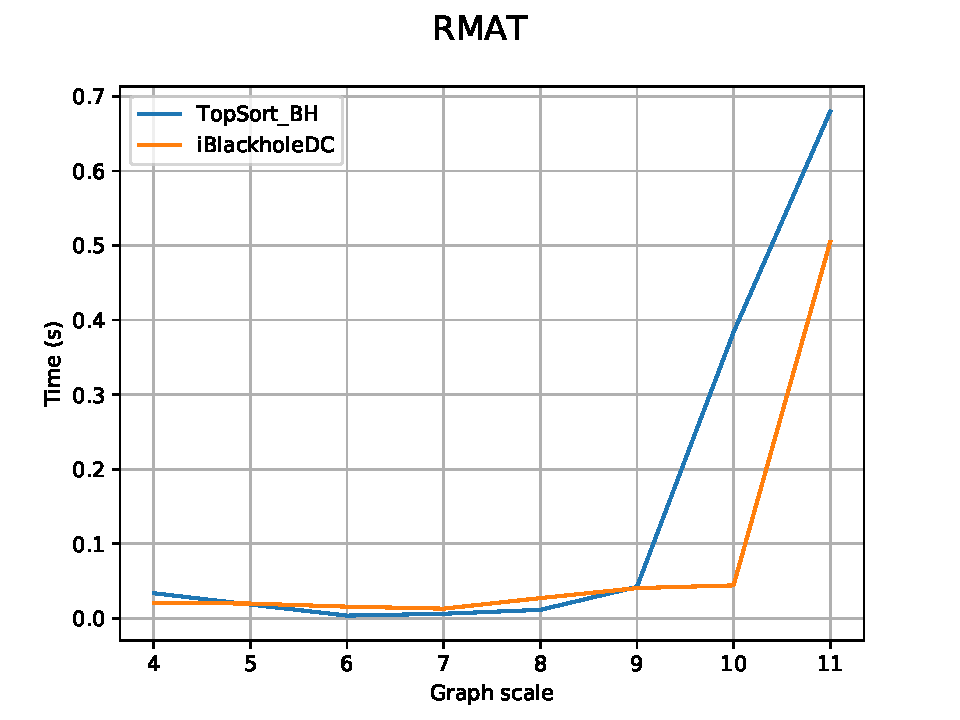
\includegraphics[width=8cm]{images/4_RMAT.pdf}
      \caption{RMAT}
      \label{fig:chinesecond:rmat}
    \end{subfigure}
    \begin{subfigure}{.5\textwidth}
      \centering
      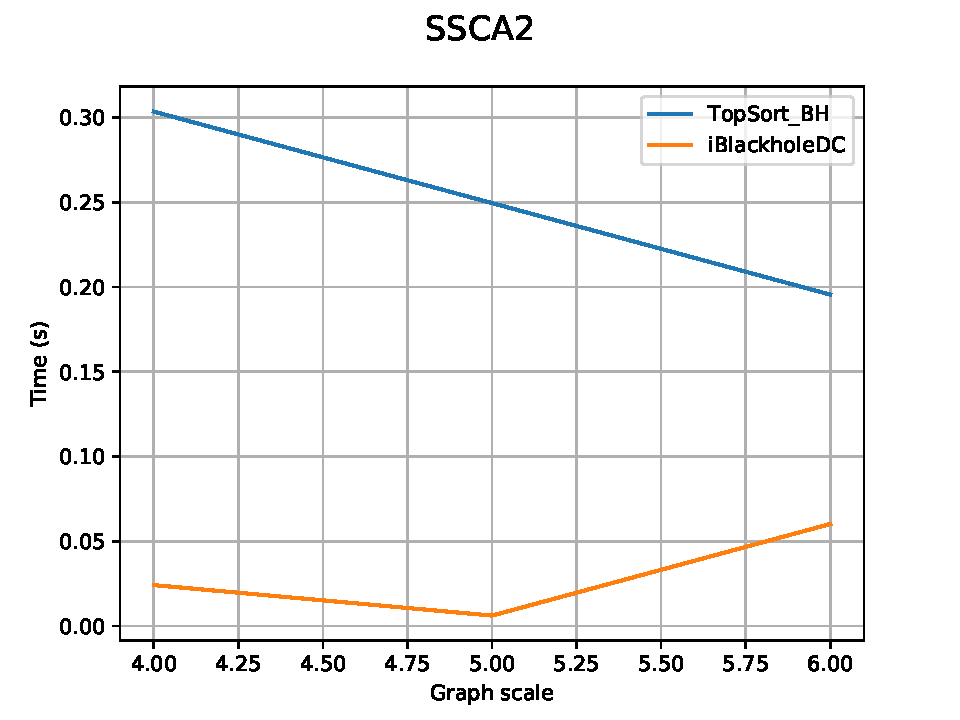
\includegraphics[width=8cm]{images/4_SSCA2.pdf}
      \caption{SSCA2}
      \label{fig:chinesecond:ssca}
    \end{subfigure}
    \begin{subfigure}{.5\textwidth}
      \centering
      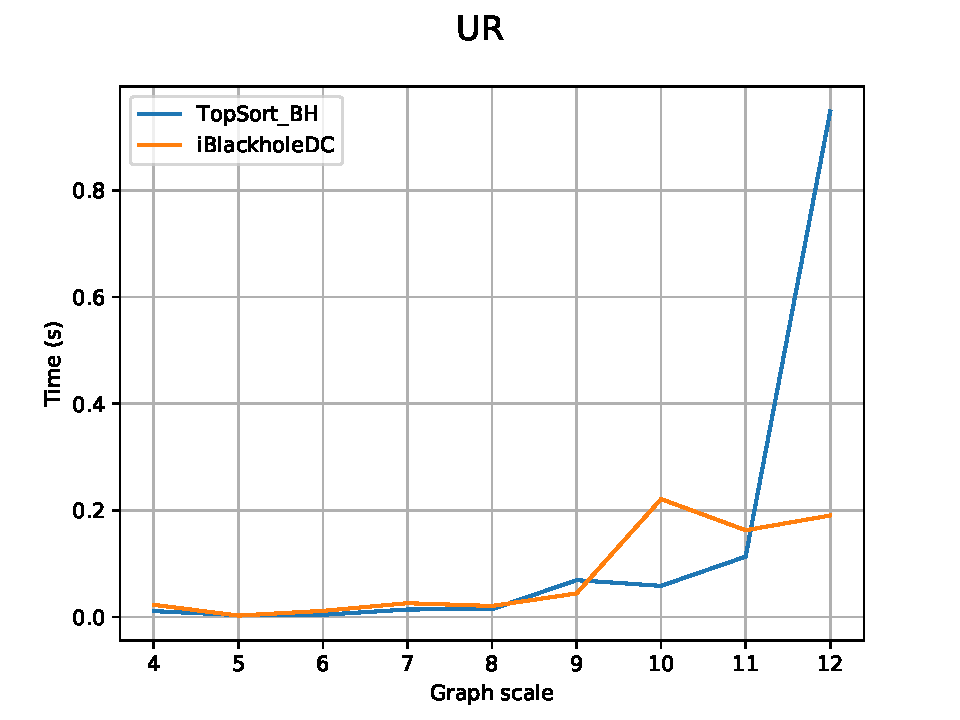
\includegraphics[width=8cm]{images/4_UR.pdf}
      \caption{UR}
      \label{fig:chinesecond:ur}
    \end{subfigure}
    \caption{Алгоритм iBlackholeDC, осуществляющий конденсацию графа перед началом своей работы,
запущен с использованием 8 потоков. Алгоритм TopSortBH запущен с использованием 8 потокoв, Timeout: 30 минут}
    \label{fig:chinesecond}
\end{figure}

Логичным шагом было добавить стадию конденсации графа в iBlackholeDC и сравнить его
многопоточный вариант с TopSortBH. Как видно на рисунке \ref{fig:chinesecond},
при таких условиях iBlackholeDC выигрывает по времени работы у TopSortBH.

\subsection{Исследование параллелизма алгоритма TopSortBH}\label{subsec:topsortasync}

\FIXME{Везде, где есть график зависимости от большого кол-ва потоков, лучше построить рядом график полученного ускорения в сравнении с линейным ускорением. Мне его не хватает, это будет более наглядное исследование параллельной эффективности реализации, а построить его легко}

\begin{figure}[H]
    \centering
    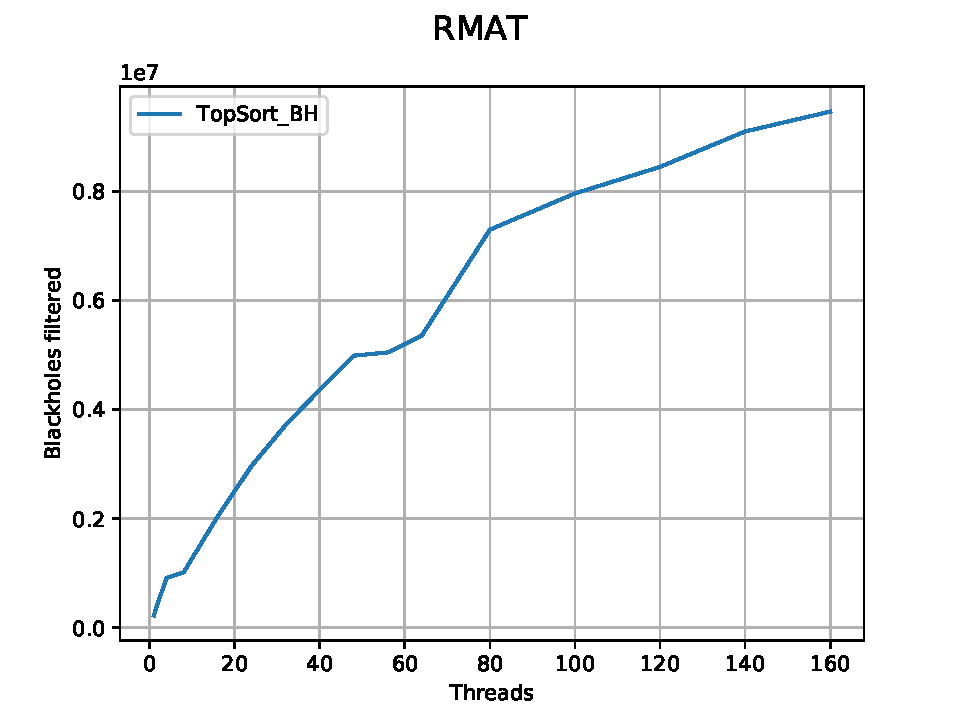
\includegraphics[width=0.8\textwidth]{images/many_threads_RMAT.pdf}
    \caption{TopSortBH запущенный с использованием от 1 до 160 потоков. По оси X отложено число потоков, по оси Y -- количество просмотренных кандидатов. Timeout: 30 минут}
    \label{fig:manythreads}
\end{figure}

\FIXME{Рисунок 9 получен с привязкой или без?}

Как уже было сказано, TopSortBH разрабатывался для использования в параллельном режиме. Поэтому
был проведен эксперимент с использованием большого количества потоков.
Все запуски производились на графе RMAT масштаба 18.
Важно отметить, что во всех конфигурациях алгоритм успел обнаружить одинаковое количество черных дыр
и завершился через полчаса работы. Поэтому было удобно сравнивать количество рассмотренных кандидатов.
Система Polus позволяет запускать до 160 потоков на одном узле, что позволило провести исследование
поведения алгоритма с использованием общей памяти.
\FIXME{Что значит 75\% результата? -- непонятная фраза} 
По графику на рисунке \ref{fig:manythreads} видно, что использование 80 потоков дает 75\%
результата, достигнутого при использовании 160 потоков. Также на графике наблюдается
заметный излом именно при 80 задействованных потоках.

\begin{figure}[H]
    \centering
    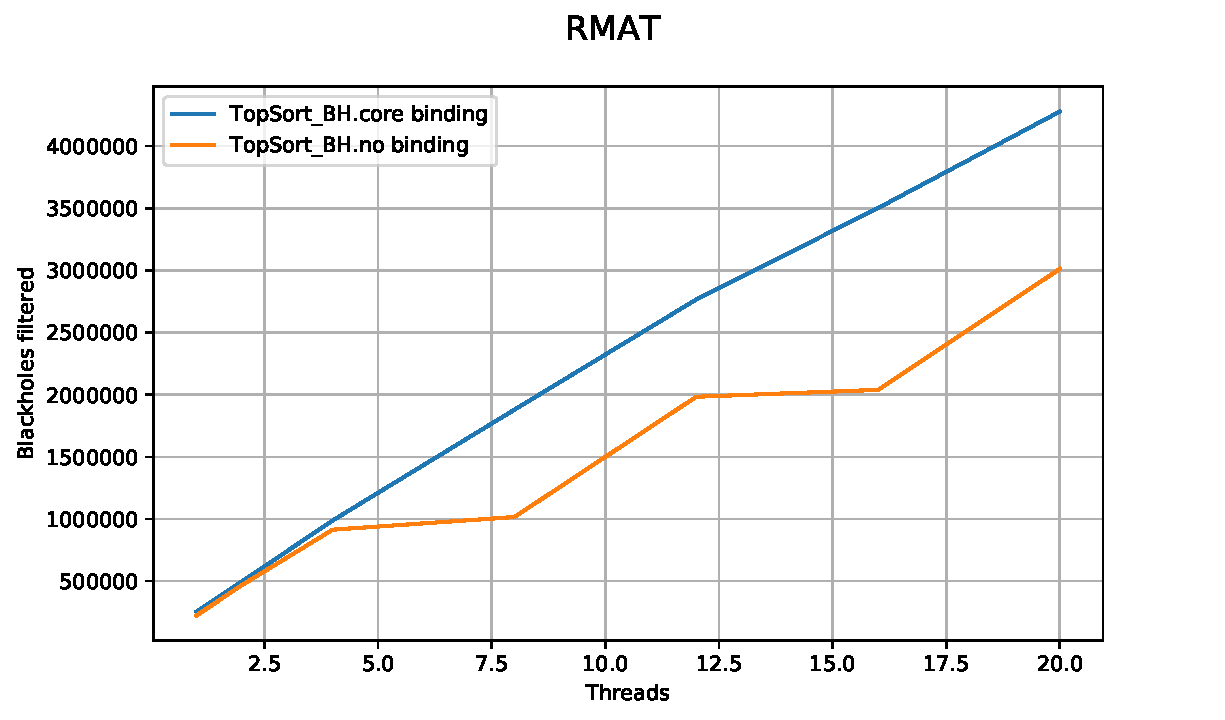
\includegraphics[width=0.8\textwidth]{images/18_threads_RMAT.pdf}
    \caption{Алгоритм TopSortBH запущенный с использованием от 1 до 20 потоков. С использованием привязки потоков и без. По оси X отложено количество потоков. По оси Y отложено число отфильтрованных кандидатов. Timeout: 30 минут}
    \label{fig:corebinding}
\end{figure}

Также алгоритм TopSortBH был протестирован в режиме привязки потоков к ядрам.
Polus располагает 20 ядрами на каждый узел, поэтому в режиме привязки было использовано не более 20 потоков.
По рисунку \ref{fig:corebinding} видно, что производительность с использованием
привязки для 20 потоков превышает результат обычного запуска на треть.
Более того 20 потоков в режиме привязки, показывают такую же производиетельность, как 40 потоков
без привязки.

\subsection{Исследование параллелизма алгоритма iBlackholeDC}\label{subsec:chinesemanythreads}

\begin{figure}[H]
    \begin{subfigure}{.5\textwidth}
      \centering
      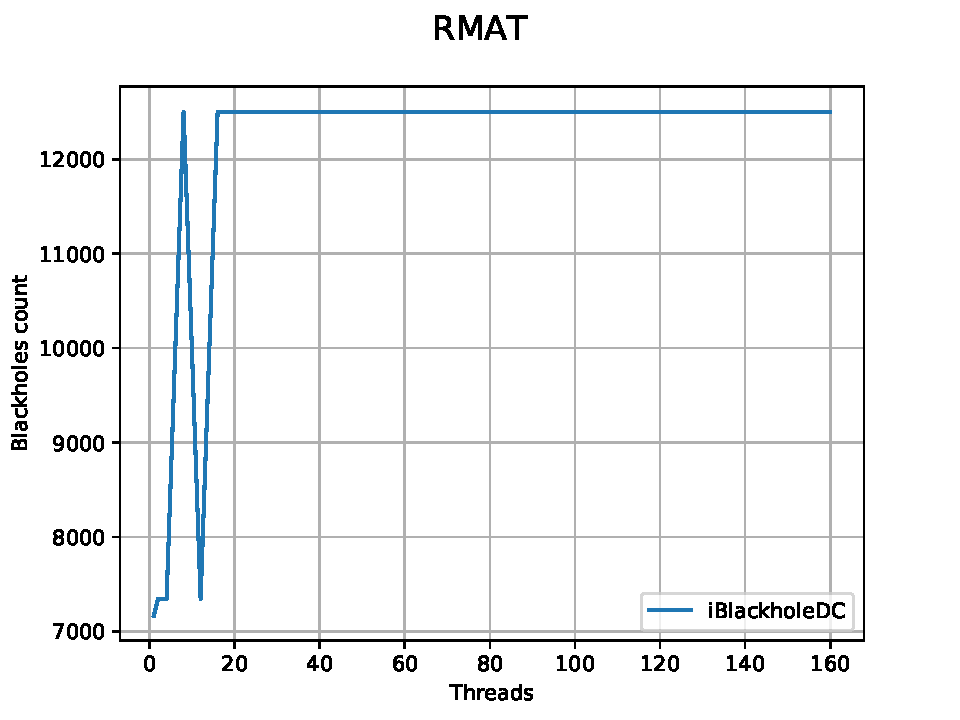
\includegraphics[width=8cm]{images/5_count.pdf}
      \caption{Обнаружено черных дыр}
      \label{fig:chinesemany:count}
    \end{subfigure}
    \begin{subfigure}{.5\textwidth}
      \centering
      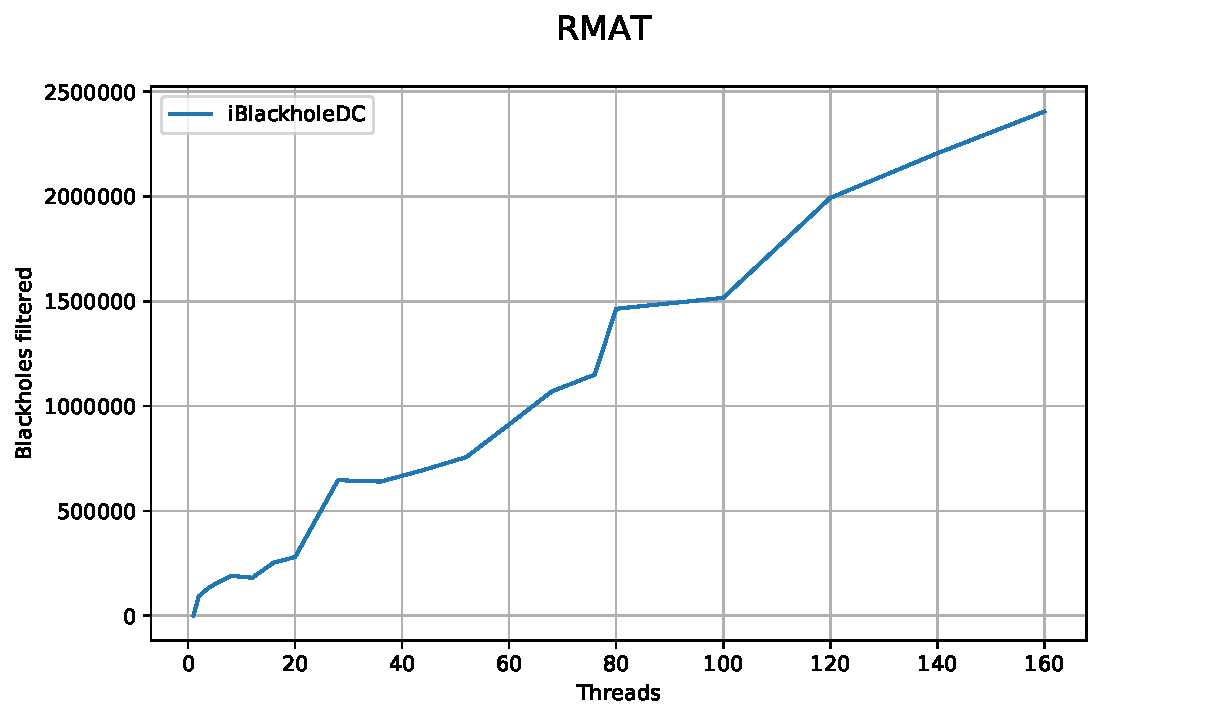
\includegraphics[width=8cm,height=6cm]{images/5_filtered.pdf}
      \caption{Отфильтровано кандидатов}
      \label{fig:chinesemany:filtered}
    \end{subfigure}
    \caption{Алгоритм iBlackholeDC запущенный для количества потоков от 1 до 160. Число потоков отложено по оси X. Timeout: 30 минут}
    \label{fig:chinesemany}
\end{figure}

Алгоритм iBlackholeDC был запущен с режиме многопоточности с использованием до 160 потоков.
Для всех запусков был установлен порог по времени 30 минут. Во время каждого запуска была собрана информация
о количестве найденных черных дыр (Рис. \ref{fig:chinesemany:count})
и количестве кандидатов, которые не прошли проверку \ref{fig:chinesemany:filtered}.
Заметим, что количество черных дыр, найденных за отведенное время, может
изменяться в зависимости от числа потоков. Такое поведение связано с
тем, что диапазон итераций, обрабатываемых каждым потоком, зависит
от номера потока и общего числа потоков.
В то же время можно отметить, что алгоритм показывает неплохую масштабируемость,
вопреки тому, что для эффективной работы следующей итерации требуется информация
о предыдущей.

\begin{figure}[H]
    \begin{subfigure}{.5\textwidth}
      \centering
      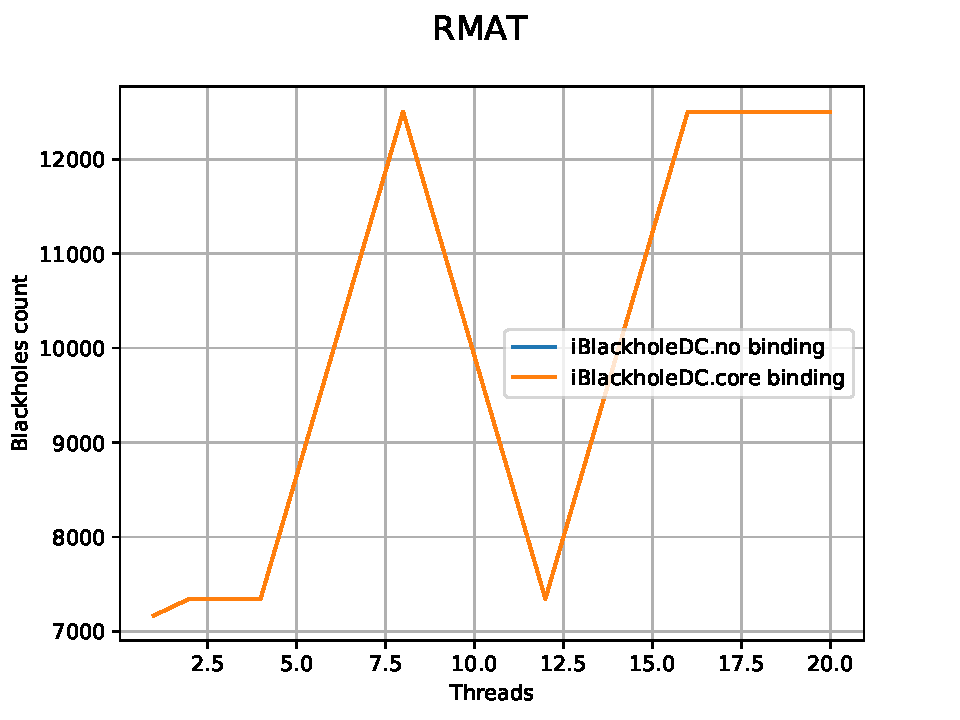
\includegraphics[width=8cm]{images/6_count.pdf}
      \caption{Обнаружено черных дыр}
      \label{fig:chinesebinding:count}
    \end{subfigure}
    \begin{subfigure}{.5\textwidth}
      \centering
      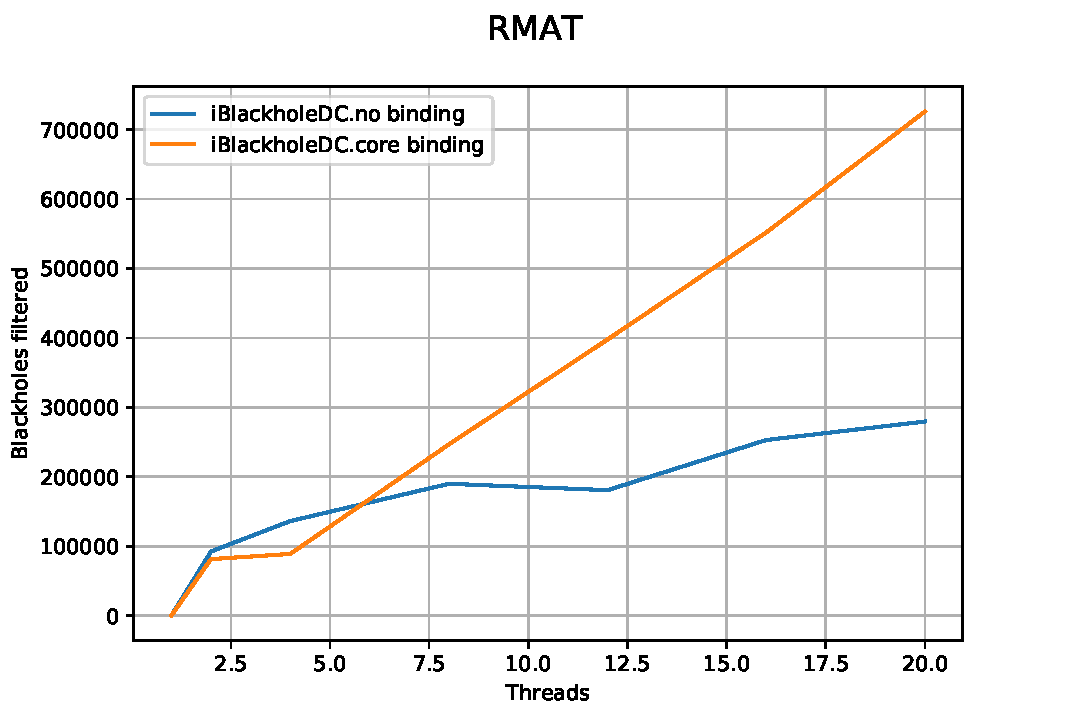
\includegraphics[width=8cm,height=6cm]{images/6_filtered.pdf}
      \caption{Отфильтровано кандидатов}
      \label{fig:chinesebinding:filtered}
    \end{subfigure}
    \caption{Алгоритм iBlackholeDC запущенный для количества потоков от 1 до 20 с использованием привязки потоков к ядру. Число потоков отложено по оси X. Timeout: 30 минут}
    \label{fig:chinesebinding}
\end{figure}

Также были проведены запуски iBlackholeDC с использованием привязки потока к ядру процессора.
Узел системы Polus имеет 2 процессора по 10 ядер, таким образом привязать можно было до  20 потоков.
На рисунке \ref{fig:chinesebinding} приведено сравнение алгоритма с использованием привязки потоков
и без. Интересен тот факт, что число обнаруженных черных дыр не меняется по сравнению с запусками без
привязки потоков. При этом значительно возрастает количество просмотренных кандидатов.

\subsection{Модификация Skip Fast}\label{subsec:fastskipexperiment}

\begin{figure}[H]
    \begin{subfigure}{.5\textwidth}
      \centering
      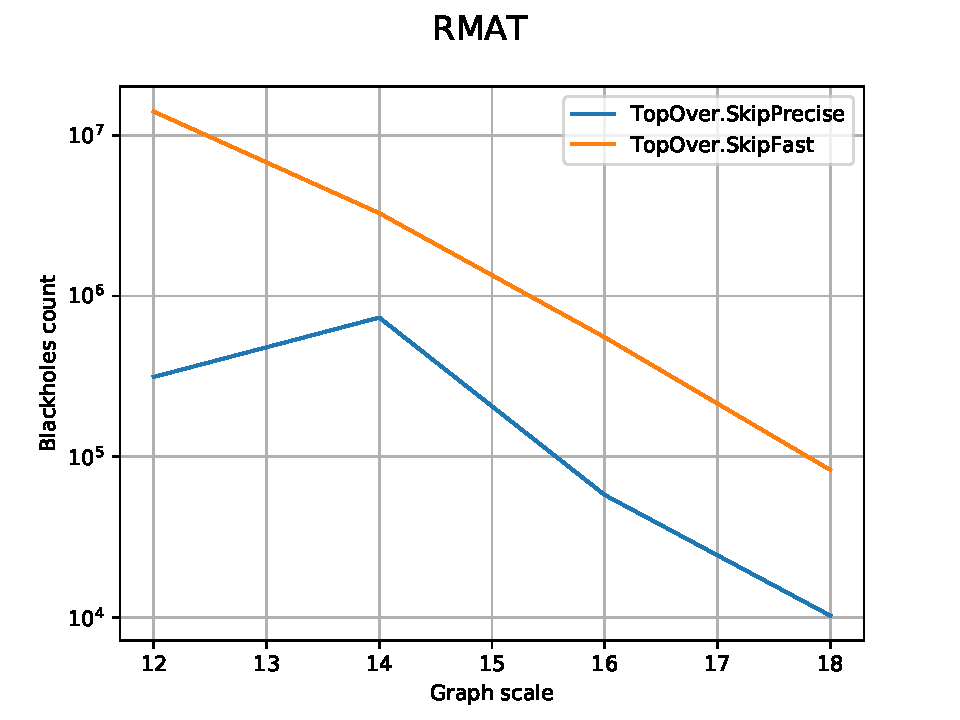
\includegraphics[width=8cm]{images/7_count_RMAT.pdf}
      \caption{Обнаружено черных дыр}
      \label{fig:fastskiprmat:count}
    \end{subfigure}
    \begin{subfigure}{.5\textwidth}
      \centering
      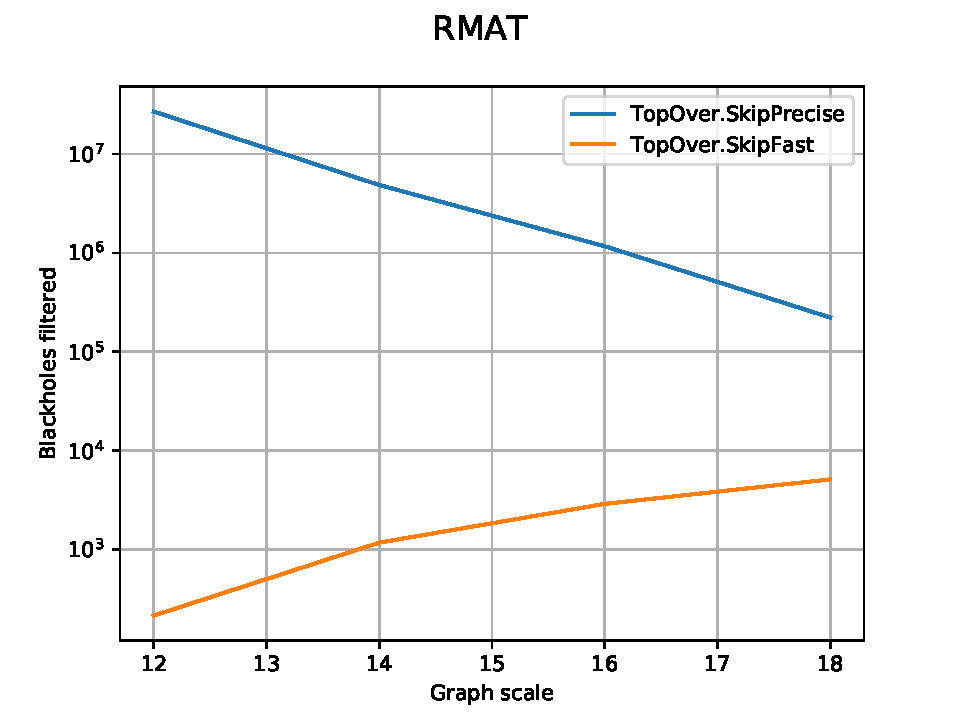
\includegraphics[width=8cm,height=6cm]{images/7_filtered_RMAT.pdf}
      \caption{Отфильтровано кандидатов}
      \label{fig:fastskiprmat:filtered}
    \end{subfigure}
    \caption{Алгоритм TopOver запущенный в 1 потоке с использованием модификации Skip Fast. По оси X отложен масштаб графа. Timeout: 30 минут}
    \label{fig:fastskiprmat}
\end{figure}

Описанная в пункте \ref{subsec:fastskip} модификация позволяет быстрее пропускать большие группы
наборов-кандидатов, но допускает появление ложно-отрицательных результатов.
В ситуациях, когда время сильно ограничено, такой подход позволяет быстрее находить черные дыры.
Данный подход был проверен экспериментально. Алгоритм TopOver был запущен в единственном потоке
на графах типа RMAT масштабом от 12 до 18 включительно. Измерялось число обнаруженных черных
дыр и число отклоненных кандидатов. При этом, применение правила Skip Fast считалось
как рассмотрение единственного кандидата, поскольку только при его рассмотрении было
затрачено время работы алгоритма.

На рисунке \ref{fig:fastskiprmat} показаны результаты данного экперимента. Видим, что за
отведенные полчаса алгоритм, использующий модификацию SkipFast, устойчиво находил на
порядок больше черных дыр, чем SkipPrecise версия. Вместе с тем, количество
рассмотренных и отклоненных кандидатов для SkipFast версии значительно уменьшилось.
Такой результат можно интерпретировать следующим образом: с большой вероятностью, оценка которой
остается за рамками данной работы, применение модификации SkipFast приводит к переходу к следующей
группе ранее не рассмотренных черных дыр.

\begin{figure}[H]
    \begin{subfigure}{.5\textwidth}
      \centering
      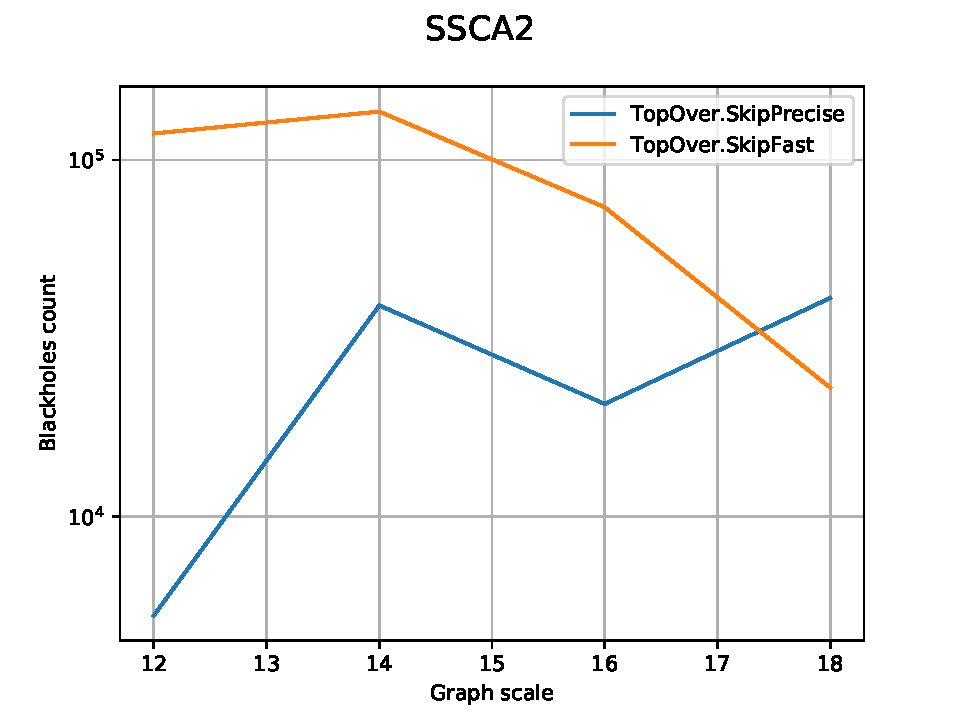
\includegraphics[width=8cm]{images/7_count_SSCA2.pdf}
      \caption{Обнаружено черных дыр}
      \label{fig:fastskipssca:count}
    \end{subfigure}
    \begin{subfigure}{.5\textwidth}
      \centering
      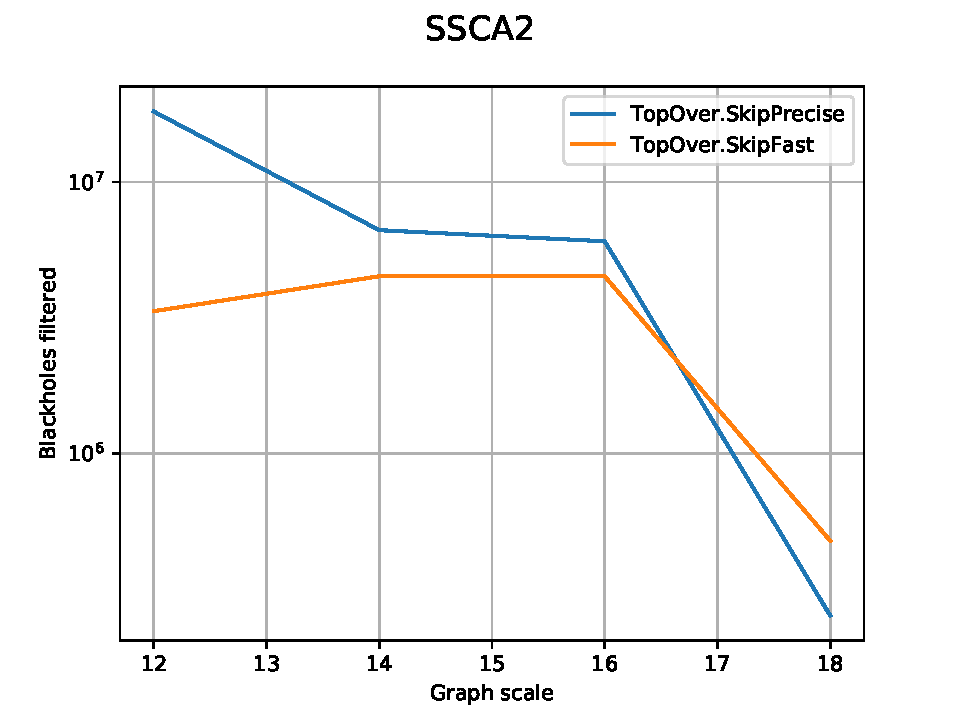
\includegraphics[width=8cm,height=6cm]{images/7_filtered_SSCA2.pdf}
      \caption{Отфильтровано кандидатов}
      \label{fig:fastskipssca:filtered}
    \end{subfigure}
    \caption{Алгоритм TopOver запущенный в 1 потоке с использованием подификации FastSkip. По оси X отложен масштаб графа. Timeout: 30 минут}
    \label{fig:fastskipssca}
\end{figure}

Также было проведено сравнение модификаций перебора SkipFast и SkipPrecise на графах SSCA2.
Здесь (см. Рисунок \ref{fig:fastskipssca}) SkipFast хорошо проявляет себя в работе с графами
масштабом до 17 включительно, но проигрывает для масштаба 18.

\FIXME{SkipFast или FastSkip? Везде должно быть одинаково}

\FIXME{На рис 15 подпись skip precise, а на рис 14 - precise. Это разные алгоритмы? Если одинаковые, тогда и подписи должны быть одинаковыми}

\begin{figure}[H]
    \begin{subfigure}{.5\textwidth}
      \centering
      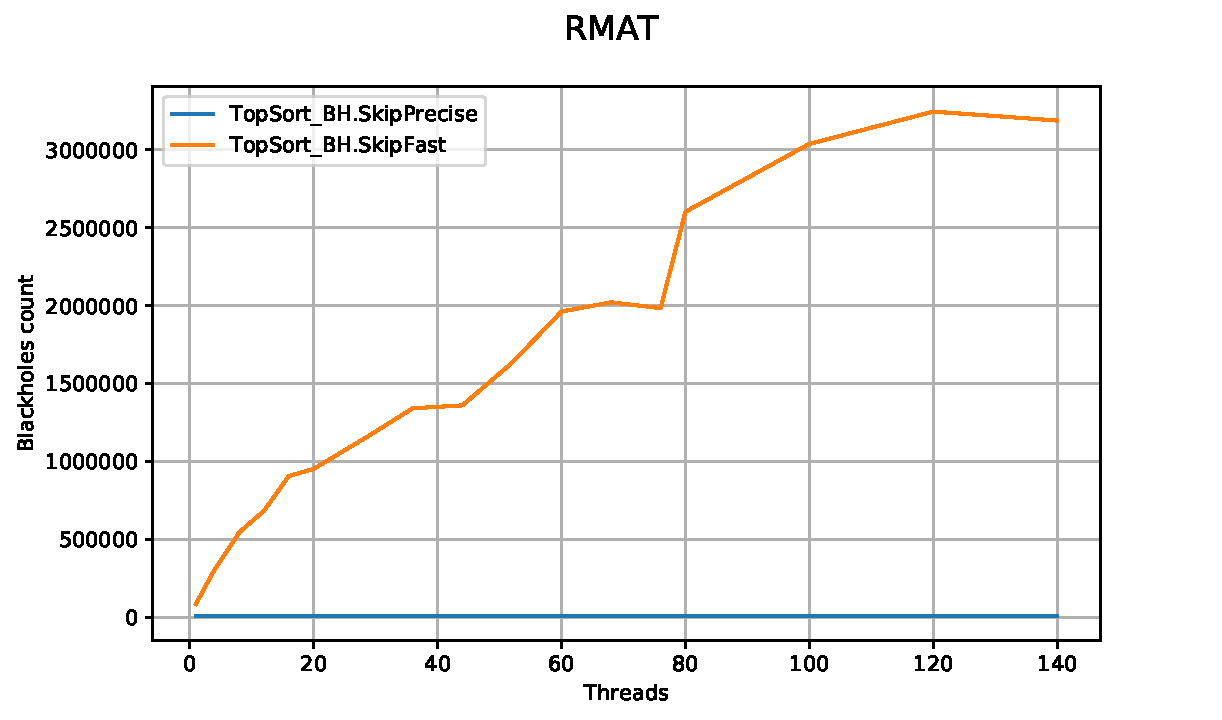
\includegraphics[width=8cm]{images/8_count.pdf}
      \caption{Обнаружено черных дыр}
      \label{fig:fastskipmanythreads:count}
    \end{subfigure}
    \begin{subfigure}{.5\textwidth}
      \centering
      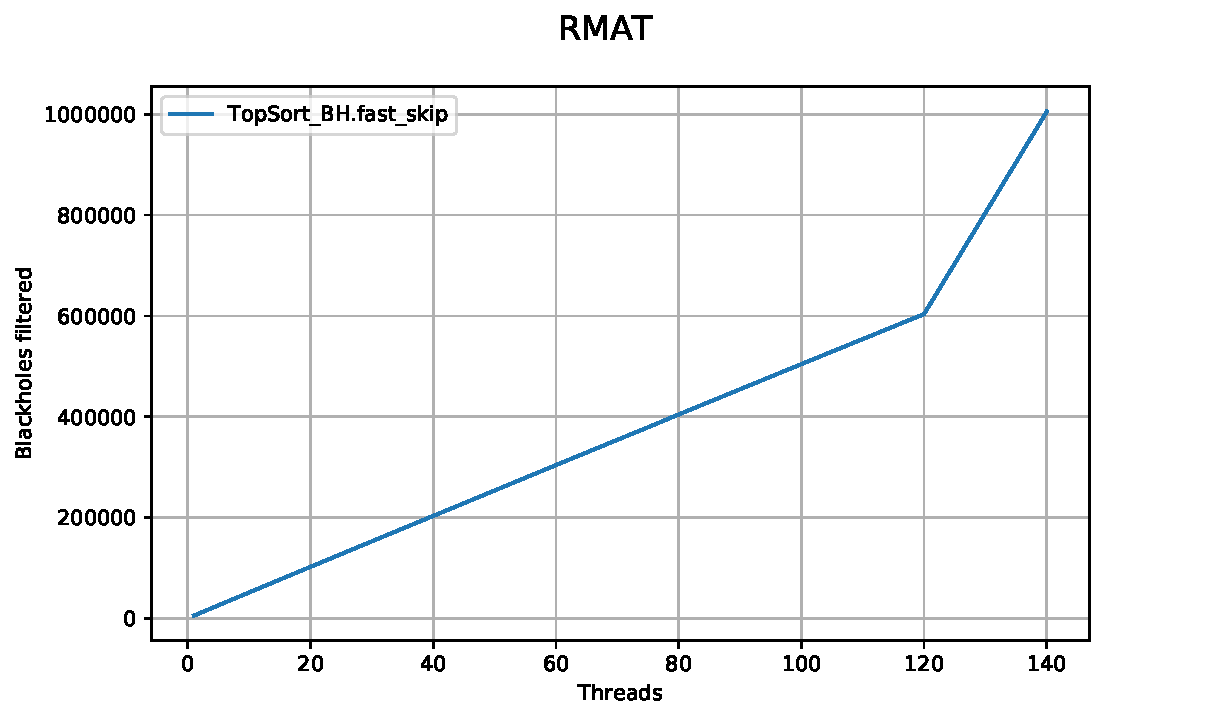
\includegraphics[width=8cm]{images/8_filtered.pdf}
      \caption{Отфильтровано кандидатов}
      \label{fig:fastskipmanythreads:filtered}
    \end{subfigure}
    \caption{Алгоритм TopSort запущенный c использованием модификации FastSkip. Число потоков от 1 до 140. Граф RMAT масштаба 18. По оси X отложено количество потоков. Timeout: 30 минут}
    \label{fig:fastskipmanythreads}
\end{figure}

Также было проверено влияение модификации SkipFast на результаты работы алгоритма
TopSortBH. Алгоритм TopSortBH был запущен на графе RMAT масштаба 18.
Запуски производились с использованием от 1 до 140 потоков. Каждый запуск был ограничен
30 минутами. Отслеживались число найденных черных дыр и число отфильтрованных кандидатов. Для сравнения,
на графиках представлены результаты работы алгоритма TopSortBH в режиме SkipPrecise,
приведенные на рисунке \ref{fig:manythreads}.

Как видно на рисунке \ref{fig:fastskipmanythreads}, TopSortBH с модификацией SkipFast
демонстрирует многократное преимущество при любом числе потоков. Причем, использование большего числа
потоков пропорционально укрепляет это преимущество. Также здесь наблюдается характерное
снижение числа отклоненных кандидатов.

\cleardoublepage
\section{Заключение}\label{sec:conclusion}
В данной работе была рассмотрена задача поиска паттерна черная дыра
в ориентированных графах без весов.

В рамках решения данной задачи был реализован предложенный ранее алгоритм iBlackhole и его модификация
iBlackholeDC. Также был разработан и реализован новый алгоритм TopSortBH.
Он состоит из трех главных частей: подход к обработке графа, ранее не
использовавшийся при решении данной задачи, подход к организации перебора,
позволяющий избегать наборов вершин, которые заведомо не являются черными дырами,
подход к сокращению такого перебора, с целью ускорения обработки графов большого размера.

В дизайне алгоритма TopSortBH заложен большой потенциал для его использования в
массивно-параллельных системах. Это было продемонстрировано с использованием общей памяти на системе Polus. \FIXME{Если результаты нормальные, лучше привести конкретное достигнутое ускорение, указав, на каком кол-во потоков оно получено}

Рассмотрено и проверено на практике комбинированное использование техник TopSortBH и iBlackhole. Такой подход назван TopOver,
и демонстрирует преимущество поиска черных дыр ограниченного размера.

Представлена и экспериментально проверена модификация SkipFast. Она позволила быстро
обнаруживать значительное количество черных дыр в условиях ограниченного времени.

\FIXME{Хотелось бы более иметь более четко сформулированные достижения, полученные в работе. Какой алгоритм обгоняет какой, на сколько. На каких графах. В чем отличие от предыдущих работ? Нет слов про большие графы. Также сформулированные здесь основные результаты должны соответствовать с формулироваками в постановке задачи. Формулировки отсюда потом пойдут в презентацию}

\FIXME{Также, на мой взгляд, стоит вынести в основные результаты информацию о том, что доказаны соответствующие теоремы в новом подходе, это придает работе более весомый вид}

%
% ---- Bibliography ----
%
\newpage
\bibliographystyle{acm}
\bibliography{biblio}
\addcontentsline{toc}{section}{Список использованных источников}

\end{document}
